% Soubory musí být v kódování, které je nastaveno v příkazu \usepackage[...]{inputenc}

\documentclass[%
%  draft,    				  % Testovací překlad
  12pt,       				% Velikost základního písma je 12 bodů
  a4paper,    				% Formát papíru je A4
  oneside,      			% Jednostranný tisk
	%twoside,      			% Dvoustranný tisk (kapitoly a další důležité části začínají na lichých stranách)
%% Z následujicich voleb lze použít maximálně jednu:
%	dvipdfm  						% výstup bude zpracován programem 'dvipdfm' do PDF
%	dvips	  						% výstup bude zpracován programem 'dvips' do PS
%	pdftex							% překlad bude proveden programem 'pdftex' do PDF (výchozí)
	unicode,						% Záložky a metainformace budou v kódování unicode
]{report}				    	% Dokument třídy 'zpráva'

\usepackage[utf8]		%	Kódování zdrojových souborů je UTF-8
	{inputenc}					% Balíček pro nastavení kódování zdrojových souborů

\usepackage[				% Nastavení okrajů
	bindingoffset=10mm,		% Hřbet pro vazbu
	hmargin={25mm,25mm},	% Vnitřní a vnější okraj
	vmargin={25mm,34mm},	% Horní a dolní okraj
	footskip=17mm,			% Velikost zápatí
	nohead,					% Bez záhlaví
	marginparsep=2mm,		% Vzdálenost poznámek u okraje
	marginparwidth=18mm,	% Šířka poznámek u okraje
]{geometry}

\usepackage{sectsty}
	%přetypuje nadpisy všech úrovní na bezpatkové, kromě \chapter, která je přenastavena zvlášť v thesis.sty
	\allsectionsfont{\sffamily}


\usepackage{graphicx} % Balíček 'graphicx' pro vkládání obrázků
											% Nutné pro vložení log školy a fakulty

\usepackage[
	nohyperlinks				% Nebudou tvořeny hypertextové odkazy do seznamu zkratek
]{acronym}						% Balíček 'acronym' pro sazby zkratek a symbolů
											% Nutné pro použití prostředí 'seznamzkratek' balíčku 'thesis'

\usepackage[
	breaklinks=true,		% Hypertextové odkazy mohou obsahovat zalomení řádku
	hypertexnames=false % Názvy hypertextových odkazů budou tvořeny
											% nezávisle na názvech TeXu
]{hyperref}						% Balíček 'hyperref' pro sazbu hypertextových odkazů
											% Nutné pro použití příkazu 'nastavenipdf' balíčku 'thesis'

\usepackage{pdfpages} % Balíček umožňující vkládat stránky z PDF souborů
                      % Nutné při vkládání titulních listů a zadání přímo
                      % ve formátu PDF z informačního systému

\usepackage{enumitem} % Balíček pro nastavení mezerování v odrážkách
  \setlist{topsep=0pt,partopsep=0pt,noitemsep}

\usepackage{cmap} 		% Balíček cmap zajišťuje, že PDF vytvořené `pdflatexem' je
											% plně "prohledávatelné" a "kopírovatelné"

%\usepackage{upgreek}	% Balíček pro sazbu stojatých řeckých písmem
											%% např. stojaté pí: \uppi
											%% např. stojaté mí: \upmu (použitelné třeba v mikrometrech)
											%% pozor, grafická nekompatibilita s fonty typu Computer Modern!

\usepackage{dirtree}		% sazba adresářové struktury

\usepackage[formats]{listings}	% Balíček pro sazbu zdrojových textů
\lstset{
%	Definice jazyka použitého ve výpisech
%    language=[LaTeX]{TeX},	% LaTeX
%	language={Matlab},		% Matlab
	language={Python},           % jazyk C
    basicstyle=\ttfamily,	% definice základního stylu písma
    tabsize=2,			% definice velikosti tabulátoru
    inputencoding=utf8,         % pro soubory uložené v kódování UTF-8
    %inputencoding=cp1250,      % pro soubory uložené ve standardním kódování Windows CP1250
		columns=fixed,  %flexible,
		fontadjust=true %licovani sloupcu
    extendedchars=true,
    literate=%  definice symbolů s diakritikou
    {á}{{\'a}}1
    {č}{{\v{c}}}1
    {ď}{{\v{d}}}1
    {é}{{\'e}}1
    {ě}{{\v{e}}}1
    {í}{{\'i}}1
    {ň}{{\v{n}}}1
    {ó}{{\'o}}1
    {ř}{{\v{r}}}1
    {š}{{\v{s}}}1
    {ť}{{\v{t}}}1
    {ú}{{\'u}}1
    {ů}{{\r{u}}}1
    {ý}{{\'y}}1
    {ž}{{\v{z}}}1
    {Á}{{\'A}}1
    {Č}{{\v{C}}}1
    {Ď}{{\v{D}}}1
    {É}{{\'E}}1
    {Ě}{{\v{E}}}1
    {Í}{{\'I}}1
    {Ň}{{\v{N}}}1
    {Ó}{{\'O}}1
    {Ř}{{\v{R}}}1
    {Š}{{\v{S}}}1
    {Ť}{{\v{T}}}1
    {Ú}{{\'U}}1
    {Ů}{{\r{U}}}1
    {Ý}{{\'Y}}1
    {Ž}{{\v{Z}}}1
}

\usepackage{float}
\usepackage{csvsimple}
\usepackage{longtable,array,ragged2e}
\usepackage{caption}
\newcommand*{\headentry}[2]{\multicolumn{1}{#1}{\centering\arraybackslash\bfseries #2}}
\newcolumntype{P}[1]{>{\RaggedRight\arraybackslash}p{#1}}
\newcolumntype{L}[1]{>{\raggedright\let\newline\\\arraybackslash\hspace{0pt}}m{#1}}
\newcolumntype{C}[1]{>{\centering\let\newline\\\arraybackslash\hspace{0pt}}m{#1}}
\usepackage{booktabs}
\usepackage{colortbl}
\usepackage{adjustbox}
\usepackage{changepage}

\newcommand*\rot{\rotatebox{45}}

\newenvironment{narrow}[2]{%
	\begin{list}{}{%
			\setlength{\topsep}{0pt}%
			\setlength{\leftmargin}{#1}%
			\setlength{\rightmargin}{#2}%
			\setlength{\listparindent}{\parindent}%
			\setlength{\itemindent}{\parindent}%
			\setlength{\parsep}{\parskip}%
		}%
		\item[]
	}{\end{list}}


%%%%%%%%%%%%%%%%%%%%%%%%%%%%%%%%%%%%%%%%%%%%%%%%%%%%%%%%%%%%%%%%%
%%%%%%      Definice informací o dokumentu             %%%%%%%%%%
%%%%%%%%%%%%%%%%%%%%%%%%%%%%%%%%%%%%%%%%%%%%%%%%%%%%%%%%%%%%%%%%%

%% Nastavení jazyka při sazbě.
% Pro sazbu češtiny je použit mezinárodní balíček 'babel', použití
% národního balíčku 'czech', ve spojení s programy 'cslatex' a
% 'pdfcslatex' není od verze 3.0 podporován a nedoporučujeme ho.
\usepackage[
%%Nastavení balíčku babel (!!! pri zmene jazyka je potreba zkompilovat dvakrat !!!)
  main=slovak,english       % originální jazyk je čeština (výchozí), překlad je anglicky
  %main=slovak,english      % originální jazyk je slovenčina, překlad je anglicky
  %main=english,czech       % originální jazyk je angličtina, překlad je česky
]{babel}    					% Balíček pro sazbu různojazyčných dokumentů; kompilovat (pdf)latexem!

\usepackage{lmodern}	% vektorové fonty Latin Modern, nástupce půvoních Knuthových Computern Modern fontů
\usepackage{textcomp} % Dodatečné symboly
\usepackage[LGR,T1]{fontenc}  % Kódování fontu -- mj. kvůli správným vzorům pro dělení slov

\usepackage[
%% Z následujících voleb lze použít pouze jednu
  %semestral,					%	sazba semestrálního práce (nesází se abstrakty, prohlášení, poděkování)
  %bachelor,					%	sazba bakalářské práce
  diploma,						% sazba diplomové práce
  %treatise,          % sazba pojednání o dizertační práci
  %phd,               % sazba dizertační práce
%% Z následujících voleb lze použít pouze jednu
% left,               % Rovnice a popisky plovoucich objektů budou %zarovnány vlevo
  center,             % Rovnice a popisky plovoucich objektů budou zarovnány na střed (vychozi)
]{thesis}   % Balíček pro sazbu studentských prací
                      % Musí být vložen až jako poslední, aby
                      % ostatní balíčky nepřepisovaly jeho příkazy


%% Jméno a příjmení autora ve tvaru
%  [tituly před jménem]{Křestní}{Příjmení}[tituly za jménem]
% Pokud osoba nemá titul před/za jménem, smažte celý řetězec '[...]'
\autor[Bc.]{Juraj}{Korček}


%% Pohlaví autora/autorky
% Číselná hodnota: 1...žena, 0...muž
\autorpohlavi{0}

%% Jméno a příjmení vedoucího/školitele včetně titulů
%  [tituly před jménem]{Křestní}{Příjmení}[tituly za jménem]
% Pokud osoba nemá titul před/za jménem, smažte celý řetězec '[...]'
\vedouci[doc.\ Ing.]{Jan}{Jeřábek}[PhD.]

%% Jméno a příjmení oponenta včetně titulů
%  [tituly před jménem]{Křestní}{Příjmení}[tituly za jménem]
% Pokud osoba nemá titul před/za jménem, smažte celý řetězec '[...]'
% Uplatní se pouze v prezentaci k obhajobě;
% v případě, že nechcete, aby se na titulním snímku prezentace zobrazoval oponent, pouze příkaz zakomentujte;
% u obhajoby semestrální práce se oponent nezobrazuje
\oponent[doc.\ Mgr.]{Křestní}{Příjmení}[Ph.D.]

%% Název práce:
%  První parametr je název v originálním jazyce,
%  druhý je překlad v angličtině nebo češtině (pokud je originální jazyk angličtina)
\nazev{Aplikace pro generování a ověřování konfigurací síťových zařízení}{Application generating and verifying configurations of network devices}

%% Označení oboru studia
% První parametr je obor v originálním jazyce,
% druhý parametr je překlad v angličtině nebo češtině
\oborstudia{Informační bezpečnost}{Information Security}

%% Označení ústavu
% První parametr je název ústavu v originálním jazyce,
% druhý parametr je překlad v angličtině nebo češtině
%\ustav{Ústav automatizace a měřicí techniky}{Department of Control and Instrumentation}
%\ustav{Ústav biomedicínského inženýrství}{Department of Biomedical Engineering}
%\ustav{Ústav elektroenergetiky}{Department of Electrical Power Engineering}
%\ustav{Ústav elektrotechnologie}{Department of Electrical and Electronic Technology}
%\ustav{Ústav fyziky}{Department of Physics}
%\ustav{Ústav jazyků}{Department of Foreign Languages}
%\ustav{Ústav matematiky}{Department of Mathematics}
%\ustav{Ústav mikroelektroniky}{Department of Microelectronics}
%\ustav{Ústav radioelektroniky}{Department of Radio Electronics}
%\ustav{Ústav teoretické a experimentální elektrotechniky}{Department of Theoretical and Experimental Electrical Engineering}
\ustav{Ústav telekomunikací}{Department of Telecommunications}
%\ustav{Ústav výkonové elektrotechniky a elektroniky}{Department of Power Electrical and Electronic Engineering}

%% Označení fakulty
% První parametr je název fakulty v originálním jazyce,
% druhý parametr je překlad v angličtině nebo v češtině
%\fakulta{Fakulta architektury}{Faculty of Architecture}
\fakulta{Fakulta elektrotechniky a~komunikačních technologií}{Faculty of Electrical Engineering and~Communication}
%\fakulta{Fakulta chemická}{Faculty of Chemistry}
%\fakulta{Fakulta informačních technologií}{Faculty of Information Technology}
%\fakulta{Fakulta podnikatelská}{Faculty of Business and Management}
%\fakulta{Fakulta stavební}{Faculty of Civil Engineering}
%\fakulta{Fakulta strojního inženýrství}{Faculty of Mechanical Engineering}
%\fakulta{Fakulta výtvarných umění}{Faculty of Fine Arts}

\logofakulta[loga/FEKT_zkratka_barevne_PANTONE_CZ]{loga/UTKO_color_PANTONE_CZ}


%% Rok obhajoby
\rok{2020}
\datum{6.\,1.\,2020} % Datum se uplatní pouze v prezentaci k obhajobě

%% Místo obhajoby
% Na titulních stránkách bude automaticky vysázeno VELKÝMI písmeny
\misto{Brno}

%% Abstrakt
\abstrakt{%
Cieľom tejto diplomovej práce je návrh a následná implementácia programu na nájdenie bezpečnostných a prevádzkových nedostatkov v sieťových zariadeniach, ako aj ich náprava pomocou generovania opravnej konfigurácie. Z dôvodu nedostatočného zabezpečenia a nesprávnej konfigurácie sú mnohé zariadenia v sieti často nevedome vystavené riziku bezpečnostného incidentu. Z tohto dôvodu program porovnáva ich nastavenia s rôznymi štandardmi, odporúčaniami a osvedčenými postupmi a vytvára správu s nálezmi, aby bolo možné tieto nedostatky odstrániť pomocou automaticky vygenerovanej nápravy alebo manuálne, pokiaľ automatická náprav nie je možná. Program využíva na nájdenie problémových nastavení regulárne výrazy, pomocou ktorých hľadá nedostatky vo vyexportovaných konfiguráciách. Jeho implementácia je v jazyku Python a využíva sa aj značkovací jazyk YAML. Vedľajším produktom práce je aj kontrolný zoznam, ktorým sa dá riadiť pri zostavovaní modulov pre podporu ďalších výrobcov, a tým rozšíriť program.
}{%
The aim of this master's thesis is a design and implementation of a program for finding security and operational deficiencies of network devices and afterwards, resolving them by generating corrective configuration. Due to a lack of security and misconfiguration, there are a lot of devices exposed to the risk of a security incident. Therefore, the program compares settings with various standards, recommendations, and best practices and generates a report with findings. Afterwards, deficiencies can be eliminated by automatic resolution or manually if automatic resolving is not possible. The program uses regular expressions to find problem settings in previously exported configurations. Implementation is written in Python, and YAML markup language is used too. Another output of this thesis is a checklist, which can be used for the creation of future modules for support of other network device vendors and thus extend the program.
}

%% Klíčová slova
\klicovaslova{%
sieť, zariadenie, smerovač, prepínač, bezpečnosť, overenie, kontrola, audit, generovanie, konfigurácia, nastavenie, python, yaml 
}{%
network, device, security, router, switch, verification, check, audit, generation, configuration, setting, python, yaml
}

%% Poděkování
\podekovanitext{%
Rád by som poďakoval vedúcemu diplomovej práce pánovi doc. Ing. Janovi Jeřábkovi Ph.D.\ za odborné vedenie, konzultácie, trpezlivosť a podnetné návrhy k~práci.
}%

% Zrušení sazby poděkování projektu SIX, pokud není nutné
%\renewcommand\vytvorpodekovaniSIX\relax  % do tohoto souboru doplňte údaje o sobě, druhu práce, názvu...

%%%%%%%%%%%%%%%%%%%%%%%%%%%%%%%%%%%%%%%%%%%%%%%%%%%%%%%%%%%%%%%%%%%%%%%%

%%%%%%%%%%%%%%%%%%%%%%%%%%%%%%%%%%%%%%%%%%%%%%%%%%%%%%%%%%%%%%%%%%%%%%%%
%%%%%%     Nastavení polí ve Vlastnostech dokumentu PDF      %%%%%%%%%%%
%%%%%%%%%%%%%%%%%%%%%%%%%%%%%%%%%%%%%%%%%%%%%%%%%%%%%%%%%%%%%%%%%%%%%%%%
%% Při vloženém balíčku 'hyperref' lze použít příkaz '\nastavenipdf'
\nastavenipdf
%  Nastavení polí je možné provést také ručně příkazem:
\hypersetup{
  pdftitle={Aplikace pro generování a ověřování konfigurací síťových zařízení},    	% Pole 'Document Title'
  pdfauthor={Bc. Juraj Korček},   	% Pole 'Author'
%  pdfsubject={Typ práce}, 						  	% Pole 'Subject'
%  pdfkeywords={Klíčová slova}           	% Pole 'Keywords'
}
%%%%%%%%%%%%%%%%%%%%%%%%%%%%%%%%%%%%%%%%%%%%%%%%%%%%%%%%%%%%%%%%%%%%%%%

\pdfmapfile{=vafle.map}

%%%%%%%%%%%%%%%%%%%%%%%%%%%%%%%%%%%%%%%%%%%%%%%%%%%%%%%%%%%%%%%%%%%%%%%
%%%%%%%%%%%       Začátek dokumentu               %%%%%%%%%%%%%%%%%%%%%
%%%%%%%%%%%%%%%%%%%%%%%%%%%%%%%%%%%%%%%%%%%%%%%%%%%%%%%%%%%%%%%%%%%%%%%
\begin{document}
\pagestyle{empty} %vypnutí číslování stránek

%% Vložení desek generovaných informačním systémem
\includepdf[pages=1]%
  {pdf/semestralka-dosky}% název souboru nesmí obsahovat mezery!
\vlozprazdnoustranku %pri dvojstrannem tisku se prida prazdna stranka
% NEBO vytvoření desek z balíčku
%\vytvorobalku
% kazdopadne ale:
\setcounter{page}{1} %resetovani citace stranek - desky se necisluji

%% Vložení titulního listu generovaného informačním systémem
\includepdf[pages=1]%
  {pdf/semestralka-titulka}% název souboru nesmí obsahovat mezery!
\vlozprazdnoustranku  %pri dvojstrannem tisku se prida prazdna stranka
% NEBO vytvoření titulní stránky z balíčku
%\vytvortitulku
   
%% Vložení zadání generovaného informačním systémem
\includepdf[pages=1]%
  {pdf/semestralka-zadanie}% název souboru nesmí obsahovat mezery!
\vlozprazdnoustranku   %pri dvojstrannem tisku se prida prazdna stranka
% NEBO lze vytvořit prázdný list příkazem ze šablony
%\stranka{}%
%	{\sffamily\Huge\centering ZDE VLOŽIT LIST ZADÁNÍ}%
%	{\sffamily\centering Z~důvodu správného číslování stránek}

%% Vysázení stránky s abstraktem
\vytvorabstrakt

%% Vysázení stránky s rozšířeným abstraktem
% (týká se pouze bc. a dp. prací psaných v angličtině, viz Směrnice rektora 72/2017)
%\cleardoublepage
%\noindent
%{\large\sffamily\bfseries\MakeUppercase{Rozšířený abstrakt}}
%\\
%Výtah ze směrnice rektora 72/2017:\\
%\emph{Bakalářská a diplomová práce předložená v angličtině musí obsahovat rozšířený abstrakt v češtině
%nebo slovenštině (čl. 15). To se netýká studentů, kteří studují studijní program akreditovaný v
%angličtině.}
%(čl. 3, par. 7)\\
%\emph{Nebude-li vnitřní normou stanoveno jinak, doporučuje se rozšířený abstrakt o rozsahu přibližně 3
%normostrany, který bude obsahovat úvod, popis řešení a shrnutí a zhodnocení výsledků.}
%(čl. 15, par. 5)


%% Vysázení prohlaseni o samostatnosti
\vytvorprohlaseni

%% Vysázení poděkování
\vytvorpodekovani

%% Vysázení obsahu
\obsah

%% Vysázení seznamu obrázků
\seznamobrazku

%% Vysázení seznamu tabulek
\seznamtabulek

%% Vysázení seznamu výpisů
\lstlistoflistings

\cleardoublepage\pagestyle{plain}   % zapnutí číslování stránek

%Pro vkládání kapitol i příloh používejte raději \include než \input
%% Vložení souboru 'text/uvod.tex' s úvodem
\chapter*{Úvod}
\phantomsection
\addcontentsline{toc}{chapter}{Úvod}


%Tato práce se věnuje oblast i \zk{zkDSP} (\zkratkatext{zkDSP}), zejména jevům, které nastanou při nedodržení Nyquistovy podmínky pro \zkratka{symfvz}.%
%\footnote{Tato věta je pouze ukázkou použití příkazů pro sazbu zkratek.}

%\begin{figure}[!h]
%	\begin{center}
%		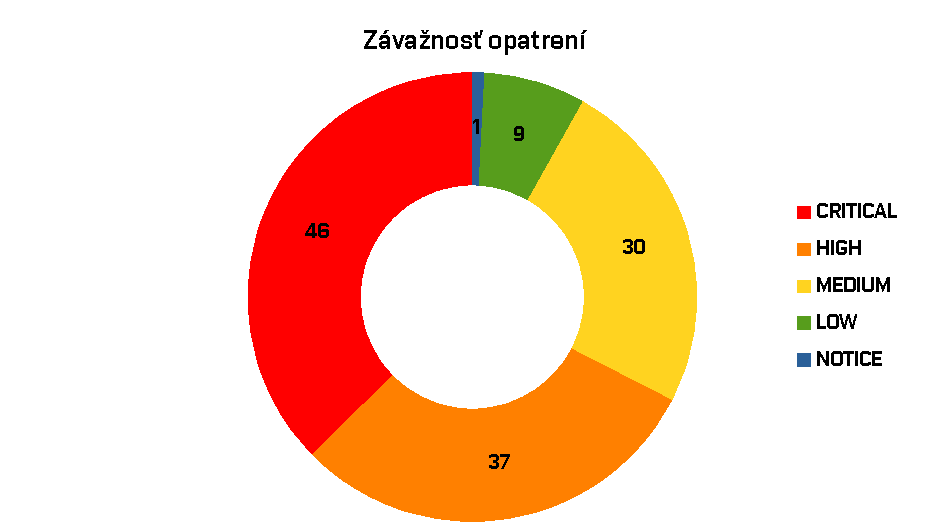
\includegraphics[scale=0.5]{obrazky/zavaznosti_graf.pdf}
%	\end{center}
%	\caption[graf_zavaznost]{Závažnosť opatrení}
%
%\end{figure}

Kybernetická bezpečnosť je bezpochyby jednou z hlavných tém 21. storočia. Útoky na infraštruktúru a systémy naberajú nielen na frekvencii, ale čo je ešte horšie na sofistikovanosti. Napriek častému zdôrazňovaniu odborníkov o kladenie čoraz väčšieho dôrazu na bezpečnosť pri návrhu, implementácii a nasadeniu, sa stále stretávame s fatálnymi dôsledkami, ktoré boli spôsobené nedostatočným venovaním pozornosti bezpečnosti. 

Problém nedostatočného zabezpečenia nie je ani tak nevedomosť základných bezpečnostných praktík administrátorov alebo programátorov, ale potreba rýchleho nasadenia systému a infraštruktúry s odložením implementácie bezpečnostných praktík na neskôr. Tieto problémy vznikajú aj pri dodatočnej implementácií nových modulov a pridaní novej infraštruktúry, kedy sa nemení celok, ale pridanie jednej časti môže výrazne ovplyvniť a zmeniť stav bezpečnosti celého systému. Z tohto dôvodu je priam žiadúce disponovať nejakým procesom alebo nástrojom na dodatočné zistenie nedostatkov a ich následnú elimináciu. Veľmi silnou motiváciou by malo byť aj to, že dôsledkom bezpečnostných nedostatkov sú globálne miliardové škody a straty reputácií firiem. 

Jednou z hlavných častí infraštruktúry, kde dochádza k významným bezpečnostným incidentom je počítačová sieť, bez ktorej by dnes informačné technológie nevedeli fungovať. Preto sa táto práca bude zaoberať práve ňou, keďže je vstupnou bránou do systémov a jej vyradením alebo zneužitím prichádzajú organizácie o finančné prostriedky, citlivé dáta a dôveru užívateľov.

Výsledkom tejto práce bude aplikácia overujúca nastavenia sieťových zariadení prevažne v lokálnej sieti, ktorá umožňuje zjednať nápravu na základe nájdených nedostatkov. Výhodou oproti existujúcim riešeniam bude otvorenosť kódu a modularita, ktorá umožní rozšírenie aplikácie na sieťové zariadenia rôznych výrobcov. Dôležitým výstupom bude taktiež zoznam bezpečnostných a prevádzkových odporučaní vychádzajúcich z rôznych štandardov a odporučaní, ktoré môžu byť v budúcnosti použité ďalšími užívateľmi aplikácie pri zostavovaní modulov pre zariadenia rôznych výrobcov. Jednou z kľúčových vlastností je bezplatnosť, keďže podľa zistení takmer polovica útokov smeruje na malé firmy, ktoré bezpečnosť často neriešia z finančnej náročnosti programov na detekciu bezpečnostných nedostatkov.    


%% Vložení souboru 'text/bezpecnost.tex' s úvodem
\chapter{Kybernetická bezpečnosť}
\phantomsection
\addcontentsline{toc}{chapter}{Kybernetická bezpečnosť}

S čoraz na väčšou informatizáciou naprieč všetkými odvetviami života, je nutnosťou riešiť aj zabezpečenie systémov, infraštruktúry a dát. Kybernetická bezpečnosť je bez pochýb jednou z najdiskutovanejších tém 21. storočia.
 
Podľa zistení z roku 2018 takmer polovica útokov smeruje na malé firmy, ktoré bezpečnosť riešia iba minimálne alebo vôbec. Predpokladá sa, že pre rok 2019 bude na kybernetickú bezpečnosť minutých 6 miliárd dolárov, naopak škody spôsobené kybernetickými útokmi presiahnu jednu miliardu dolárov a veľmi záškodné útoky typu \zkratka{zkDDoS} by mali vzrásť až šesťnásobne. \cite{Milkovich3122018} 

Vyššie zmienené predpovede len potvrdzujú dôležitosť kybernetickej  bezpečnosti pri návrhu, implementácie, nasadzovaní a prevádzke informačných technológií.




\section{Vybrané pojmy z kybernetickej bezpečnosti}
\begin{itemize}
	\item Informačné aktívum (Asset)\,--\,čokolvek, čo je nutné chránit, napr. dáta, fyzická informačná infraštruktúra, systémy \cite{McMillan2018}.\\
	
	\item Zraniteľnosť (Vulnerability)\,--\,neprítomnosť alebo nedostatočné opatrenia na zabezpečenie. Zraniteľnosť môže byť prítomná hardvéri, softvéri alebo samotnom užívateľovi \cite{McMillan2018}.\\
	
	\item Hrozba (Threat)\,--\,vzniká v prípade odhalenia alebo zneužitia zraniteľnosti. Zároveň platí, že hrozbou je aj zraniteľnosť, ktorá doposiaľ nebola neidentifikovaná \cite{McMillan2018}.\\
	
	\item Útočník (Threat agent)\,--\,entita, ktorá zneužije zraniteľnosť \cite{McMillan2018}.\\
    
    \item Riziko (Risk)\,--\,pravdepodobnosť, že útočník využije zraniteľnosť, pričom príde k dopadu na systém alebo infraštruktúru \cite{McMillan2018}.\\
  	
  	\item Útok na bezpečnosť (Security attack/Explotation)\,--\,krok, ktorý kompromituje bezpečnosť informačného aktíva \cite{Vyncke2008}.\\
  	    
	\item Bezpečnostný mechanizmus (Security mechanism)\,--\,proces, ktorý je navrhnutý na detegovanie, prevenciu a zotavenie z útoku na bezpečnosť. \\
	
	\item Protiopatrenie (Countermeasure)\,--\,ochranné opatrenie, ktoré znižuje riziko \cite{McMillan2018}.\\
	
	\item Expozícia informačného aktíva (Exposure)\,--\,dochádza k nej ak je aktívum vystavené stratám nedostatočným alebo neprítomným zabezpečením \cite{McMillan2018}.\\
	
\end{itemize}

	\begin{figure}[!h]
	\begin{center}
		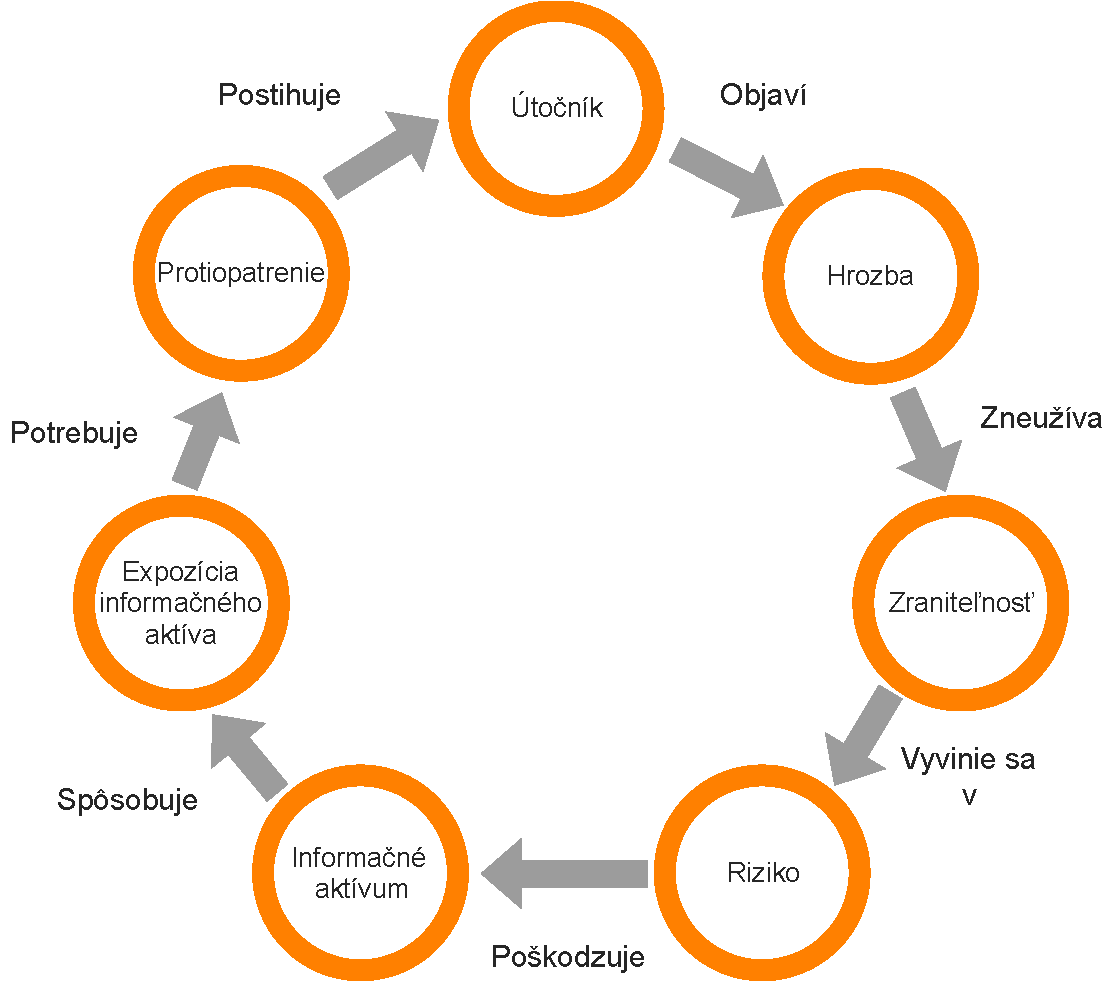
\includegraphics[scale=0.5]{obrazky/sec_cycle.pdf}
	\end{center}
	\caption[Koncept bezpečnosti a vzájomné vzťahy pojmov]{Koncept bezpečnosti a vzájomné vzťahy pojmov \cite{McMillan2018}}
	\label{sec-cycle}
	\end{figure}

Na obrázku \ref{sec-cycle} je možné vidieť vzájomnú interakciu medzi pojmami. Zároveň je nutné si uvedomiť, že takýto cyklus nie je v systéme alebo infraštruktúre jeden a taktiež môže vzniknúť niekoľko paralelných cyklov pričom každý môže mať počiatok v inom uzle. Je dobré myslieť na to, že jednotlivé cykly môžu na seba vplývať, napríklad jedno protiopatrenie môže postihnúť viacero útočníkov využívajúcich rôzne hrozby. 

\


\section{Ciele sieťovej bezpečnosti}
Bezpečnosť počítačovej siete, tak ako aj iných podoblastí kybernetickej bezpečnosti je založená na troch základných princípoch známych ako \zkratka{zkCIA}. Bezpečnosť musí pokryť všetky tri aspekty popísané týmto modelom, pričom narušenie čo i len jednej zložky má za následok nesplnenie celkového zabezpečenia \cite{Vyncke2008}. 

\subsection{Triáda CIA}

\begin{itemize}
	\item Confidentiality (Dôvernosť)\,--\,zabránenie prístupu k dátam alebo informáciám neoprávneným osobám. Na zaistenie tejto požiadavky sa najčastejšie používa šifrovanie, ale aj autentizácia a autorizácia. Jej strata vedie k neoprávnenému zverejnenie informácií. \cite{McMillan2018}
	
	\item Integrity (Integrita)\,--\,dáta alebo informácie sú zabezpečené proti neautorizovanej modifikácií a poškodeniu. Týmto zaisťujem konzistenciu dát pri prenose alebo uchovaní na médiu. Integritu zaisťujeme hašovacími funkciami prípadne za pomoci \zkratka{zkACL}. \cite{McMillan2018}
	
	\item Availability (Dostupnosť)\,--\,dáta alebo informácie sú dostupné iba pre určité entity v daný čas a miesto. \cite{McMillan2018}

	\begin{figure}[!h]
		\begin{center}
			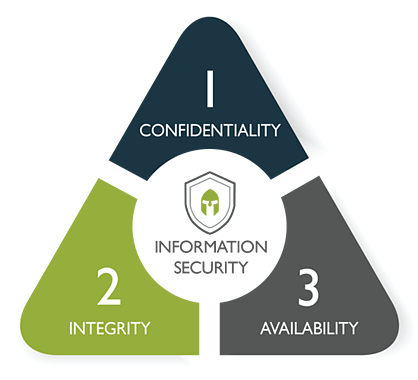
\includegraphics[scale=0.3]{obrazky/cia.png}
		\end{center}
		\caption[Triáda CIA]{CIA triáda\footnotemark}				\label{cia}
	\end{figure}\footnotetext{Zdroj: https://www.comtact.co.uk/blog/what-is-the-cia-triad}
\end{itemize}

	Aj keď triáda \zk{zkCIA} definuje ciele na zaistenie bezpečnosti, tak niektorí odborníci ju nepovažujú za dostatočnú a zavádzajú ďalšie dve podmienky a pojmy:\\
	\\
	\begin{itemize}
		\item Authencity (Autenticita)\,--\,overenie originálnosti a platnosti správy a identity jej pôvodcovi. Najčastejšie sa na zaistenie tejto podmienky využívajú certifikáty. \cite{Stallings2011}
		\item Accountability (Sledovateľnosť)\,--\,identifikácia prístupu k informáciám a vysledovateľnosť bezpečnostných incidentov v prípade využitia forenznej analýzy. Väčšinou je táto požiadavka zaistená záznamom činnosti v systéme formou logu. \cite{Stallings2011}
	\end{itemize}





\newpage
\section{Pasívne a aktívne útoky}
Útoky na bezpečnosť môžu byť rozdelené do dvoch skupín. Jednou skupinou je pasívny útok, kde nepozmeňuje útočník pôvodné dáta a nevplýva na príjemcu týchto dát. Druhou možnosťou je aktívny útok, pri ktorom sú buď pozmenené dáta doručené príjemcovi alebo je obeť nejakým spôsobom ovplyvňovaná, napríklad zasielaním falošných informácií. \cite{Vyncke2008}

\begin{figure}[H]
	\begin{center}
		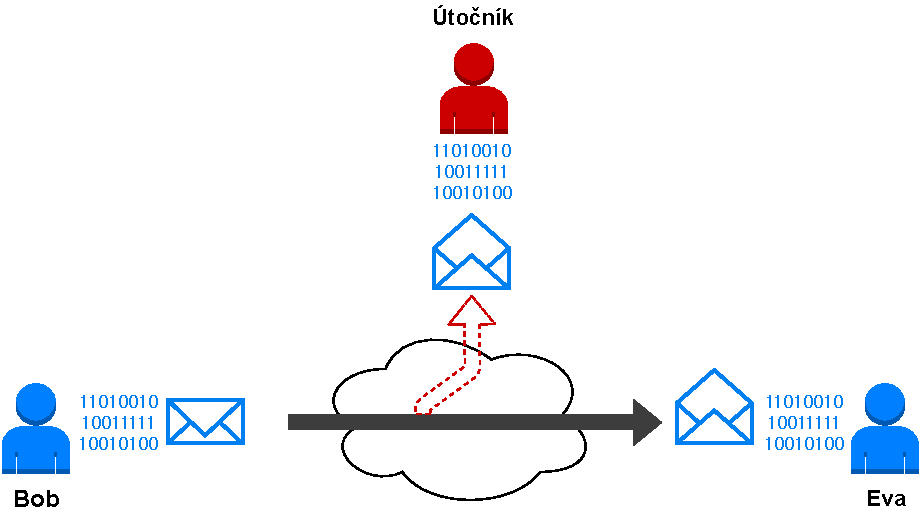
\includegraphics[scale=0.65]{obrazky/passive-attack.pdf}
	\end{center}
	\caption[Pasívny útok]{Pasívny útok}
	\label{passive-attack}
\end{figure}

Pri pasívnom útoku, ktorý je znázornený na obrázku \ref{passive-attack} ide útočníkovi prevažne o zachytenie prenášanej komunikácie a monitorovanie a  analýzu prevádzky. Odposluch a zobrazenie obsahu dát je účinné hlavne pri nepoužití šifrovania správ medzi koncovými bodmi alebo aj pri použití slabých šifier, krátkych kľúčov a nedostatočne bezpečných hesiel. Monitorovanie prevádzky, respektíve analýza komunikácie je možná aj pri použití šifrovania, keďže každá komunikácia je charakteristická určitým vzorom. Pasívne útoky je nesmierne obtiažne detegovať nakoľko nemodifikujú dáta pri prenose. Najúčinnejšia obrana je použitie dostatočne silných šifier na zabezpečenie dát. Jeden z pasívnych útokov sa hojne využíva aj pri prevencii v \zkratka{zkIDS} a \zkratka{zkIPS}, kde bez analýzy prevádzky by nebolo možné zabezpečiť sieť. Pasívnymi útokmi sa nespôsobuje škoda na systéme alebo infraštruktúre, ale hrozba spočíva v narušení dôvernosti.

\begin{figure}[H]
	\begin{center}
		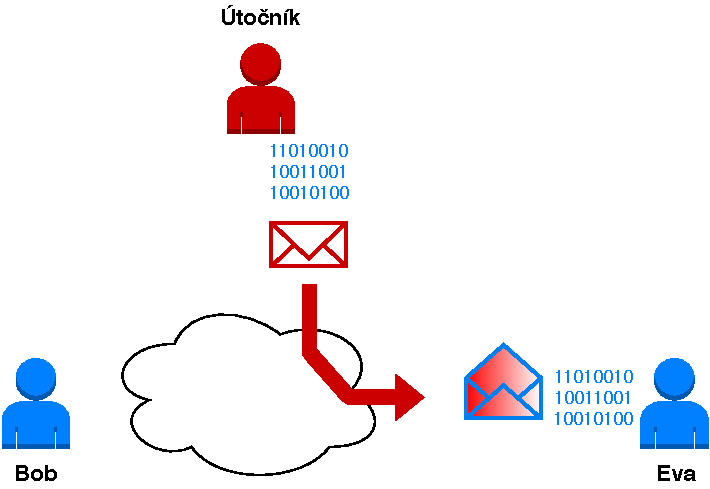
\includegraphics[scale=0.65]{obrazky/active-attack-masq.pdf}
	\end{center}
	\caption[Aktívny útok maškaráda]{Aktívny útok maškaráda}
	\label{active-attack-masq}
\end{figure}

\begin{figure}[H]
	\begin{center}
		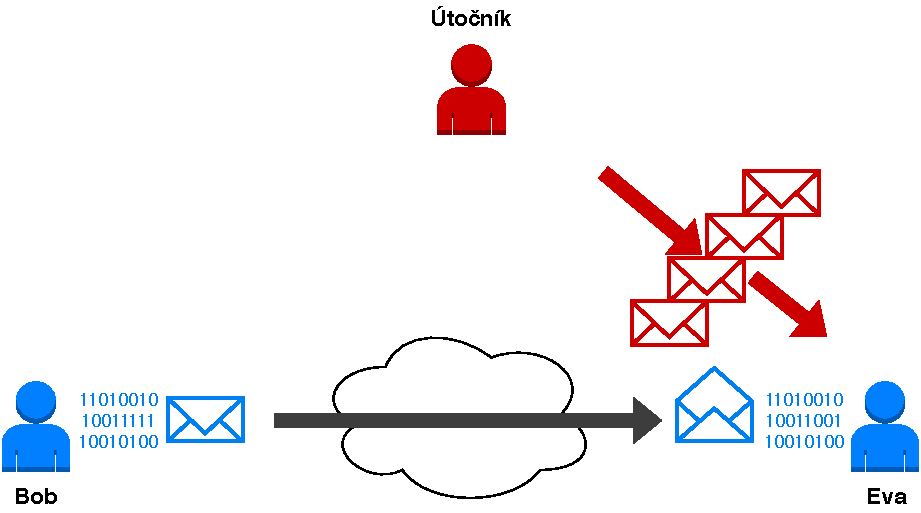
\includegraphics[scale=0.65]{obrazky/active-attack-dos.pdf}
	\end{center}
	\caption[Aktívny útok DOS]{Aktívny útok DOS}
	\label{active-attack-dos}
\end{figure}

\begin{figure}[H]
	\begin{center}
		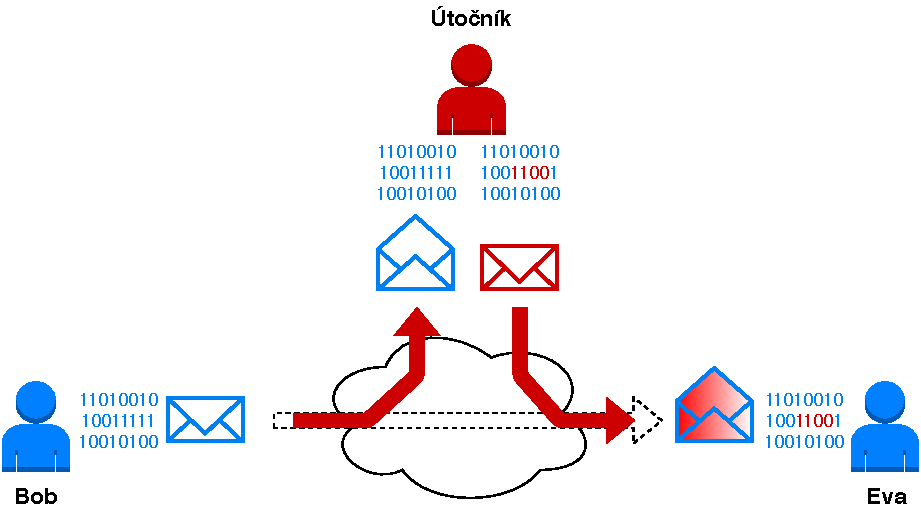
\includegraphics[scale=0.65]{obrazky/active-attack-mod.pdf}
	\end{center}
	\caption[Aktívny útok modifikácia správy]{Aktívny útok modifikácia správy}
	\label{active-attack-mod}	
\end{figure}

\begin{figure}[H]
	\begin{center}
		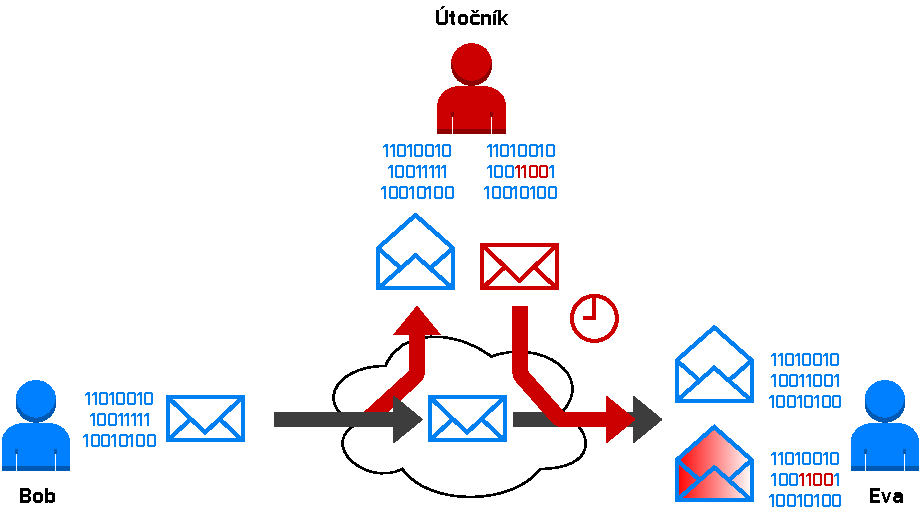
\includegraphics[scale=0.65]{obrazky/active-attack-reply.pdf}
	\end{center}
	\caption[Aktívny útok prehratím]{Aktívny útok prehratím}
	\label{active-attack-reply}
\end{figure}

Aktívne útoky sú sofistikovanejšie ako pasívne, modifikujú dáta alebo vytvárajú falošné, o ktorých prijímateľ predpokladá, že prišli od zdroja, s ktorým pôvodne komunikoval. Hrozby, ktoré môžu týmito útokmi nastať sú strata integrity, teda modifikácia dát a ohrozenie dostupnosti pričom vždy dochádza ku škode na systéme alebo infraštruktúre. Maškaráda je prvým z aktívnych útokov, kde ako je možné vidieť na obrázku \ref{active-attack-masq}, útočník vytvára falošnú správu, ktorú zasiela obeti a tá sa domnieva, že komunikuje s pôvodným zdrojom, v našom prípade Bobom. Príkladom aktívneho útoku je aj útok odoprenia služby \ref{active-attack-dos}, kde sa vytvárajú falošné dáta generované vysokou frekvenciou za účelom odstaviť systém alebo infraštruktúru, ktorá nezvláda spracovanie toľkých požiadaviek, keďže nebola na takúto záťaž dimenzovaná. Tretím aktívnym útokom \ref{active-attack-mod} je modifikácia správy útočníkom pri prechode komunikačným kanálom, ktorý sa realizuje rôznymi technikami podvrhnutia zdroja alebo identity. Posledným útokom je útok prehratím \ref{active-attack-reply}, čo je útok veľmi podobný predchádzajúcemu, akurát obeť obdrží najprv pôvodnú nepozmenenú správu a následne po určitom čase aj modifikovanú správu od útočníka.  






%% Vložení souboru 'text/bezpecnostny-audit.tex' s úvodem
\chapter{Bezpečnostný audit}
\label{bezpecnostny-audit}
\phantomsection

Audit je veľmi dôležitým prvkom správy informačných systémov a infraštruktúry, pretože umožňuje zaistiť bezpečnosť týchto informačných aktív porovnávaním s~vytvorenými štandardmi, odporúčaniami a predpismi. Zaoberá sa otázkami čo a ako zabezpečiť, vyhodnocovaním a riadením rizík a následným dokazovaním, že náprava znížila riziko hrozby.
\\\\
\noindent
Audit sa skladá z~piatich pilierov \cite{Jackson2010}:

\begin{enumerate}
	\item Posúdenie
	\item Prevencia
	\item Detekcia
	\item Reakcia
	\item Zotavenie
\end{enumerate}

\vspace{1em}
\noindent
Pri posudzovaní si je potreba klásť otázky či sú prístupové práva dostatočne špecifikované, aká je pravdepodobnosť útoku na zraniteľnosť a podobne. Prevencia nespočíva iba v~technológiách ako firewall prípadne \zk{zkIDS} a \zk{zkIPS}, ale aj v~politikách, procesoch a povedomí o~probléme. Detekcia a reakcia spolu úzko súvisia a je potrebné skrátiť dobu medzi týmito dvoma bodmi, bez dôkladnej detekcie nie je možné vykonať reakciu.	Mnohé reakcie na detekciu problému sú už rôznymi technológiami implementované automatizovane. Posledný článkom je zotavenie, ktoré je dôležité pri službách vysokej dostupnosti. Výborným príkladom detekcie, reakcie a zotavenia z~problému sú protokoly z~rodiny \zkratka{zkFHRP}.

\vspace{1em}
\noindent
Proces auditu pozostáva z~niekoľkých fáz: \cite{Jackson2010} 
\begin{enumerate}
	\item Plánovanie\,--\,stanovenie cieľov a predmetu auditu. Definuje sa rozsah, teda čo všetko je v~pláne auditom pokryť. 
	\item Výskum\,--\,vytváranie auditného plánu na základe štandardov a odporúčaní a špeciálnych expertíz. Kontaktujú sa tiež dotknuté strany, ktoré nám môžu byť nápomocné pri plnení cieľov.
	\item Zbieranie dát\,--\,vyžiadanie potrebných podkladov a dát na vykonanie auditu, zozbieranie dôkazov. V~tejto fáze sa tiež vyberajú rôzne softvérové nástroje na vykonanie auditu a vytvorí sa kontrolný zoznam na základe auditného plánu a zozbieraných dôkazov.  
	\item Analýza dát\,--\,posúdenie všetkých dôkazových dát pomocou kontrolného zoznamu a softvéru na podporu auditu. Na základe nájdených nedostatkov sa vytvoria odporúčania, ktoré by mali znížiť riziká hrozieb.
	\item Vytváranie správy\,--\,súpis nájdených nedostatkov, možných riešení na zníženie rizík do auditnej správy a prezentácia tejto správy dotknutým stranám.
	\item Aplikácia opatrení\,--\,nasadenie a použitie protiopatrení prezentovaných alebo vyplývajúcich z~auditnej správy. Následne sa môže vykonať monitorovanie a hlásenie o~úspešnosti zmien.
\end{enumerate}

\vspace{1em}
\noindent
Typy auditov podľa zistení, hĺbky a rozsahu auditu:
\begin{itemize}
	\item Bezpečnostná kontrola\,--\,je najzákladnejšia forma analýzy bezpečnosti, na základe ktorej sa následne formujú ďalšie aktivity na zaistenie bezpečnosti. Do tejto kategórie spadajú automatizované nástroje na skenovanie zraniteľností a penetračné nástroje, ktoré generujú zoznam potenciálnych zraniteľností, ale je potrebné ďalšie podrobnejšie preskúmanie výsledkov a zistení a stanovenie, ako sa k~ním zachovať. Patria sem nástroje ako napríklad Nmap, Nessus a podobne. Za bezpečnostnú kontrolu možno považovať preskúmanie politík alebo architektúry daného systému a infraštruktúry. Dá sa povedať, že ide o~akýsi rýchly náhľad na bezpečnosť, ktorého výstupom je poznanie a identifikovanie problému.
	\item Hodnotenie bezpečnosti\,--\,je ďalším stupňom, pričom ide o~podrobnejší pohľad na problém z~profesionálnejšieho hľadiska. Kvalifikuje sa riziko k~jednotlivým zisteniam a stanovuje sa relevantnosť a kritickosť týchto zistení na konkrétnu organizáciu a prípad použitia.
	\item Bezpečnostný audit\,--\,je štandardizovanou a najdôkladnejšou formou posúdenia bezpečnosti. Bezpečnosť sa porovnáva so štandardmi alebo benchmarkmi, v~niektorých prípadoch aj s~predpismi dohliadajúcich orgánov. Výsledkom je posúdenie, na koľko je organizácia alebo skúmaný objekt v~zhode s~porovnávaným štandardom. Typickým príkladom štandardov sú ISO27001 a COBIT.
\end{itemize}

\section{Manažment rizík}
\label{riskmanagement}
Manažment rizík je proces pozostávajúci z~analýzy rizík a riadenia rizík \cite{McMillan2018}. Dôležitým faktom je, že riziko nie je možné eliminovať, ale ho iba znížiť.

Pri analýze rizík zisťujeme, aké riziká existujú, ako medzi sebou súvisia a aké škody môžu spôsobiť. Analýza rizík môže byť vykonávaná kvalitatívne a kvantitatívne.\\ 
\newpage
\noindent
Štandard NIST SP 800-30 \cite{7TVhmfuQFbsOANAz} definuje nasledujúce kroky pri analýze rizík:

\begin{enumerate}
	\item Identifikácia informačných aktív a ich význam
	\item Identifikácia hrozieb
	\item Identifikácia zraniteľností
	\item Analýza riadenia a kontroly 
	\item Zistenie pravdepodobnosti
	\item Identifikovanie dopadu
	\item Definovanie rizika ako súčinu pravdepodobnosti a dopadu
	\item Odporúčanie na zavedenie riadenia a kontroly na zníženie rizika  
	\item Zdokumentovanie výsledkov
\end{enumerate} 
\vspace{2em}
Riadenie rizík má za úlohu minimalizáciu potenciálnych škôd odhalených pri analýze rizík s~ohľadom na vyváženie nákladov na riadenie rizika. 
\\\\
\noindent
Prístupy k~nájdenému riziku \cite{Vyncke2008}\cite{McMillan2018}\cite{Jackson2010}:
\begin{itemize}
	\item Vyhnutie sa riziku\,--\,je uplatnené ak prítomnosť a funkčnosť informačného aktíva nestojí za podstúpenie rizika, a teda toto aktívum vôbec nepoužijeme. Napríklad vypnutie menej bezpečných a nevyužívaných sieťových služieb.  
	
	\item Zníženie\,--\,aplikovanie protiopatrenia na odstránenie hrozby alebo zraniteľnosti prípadne zníženie pravdepodobnosti rizika. Nikdy nie je však možné riziko eliminovať. Príkladom môže byť obmedzenie prístupu k~sieťovému prvku.
	
	\item Akceptovanie\,--\,v prípade neexistujúceho protiopatrenia alebo veľmi nízkeho rizika. Častokrát ide o~bezpečnostnú chybu softvéru v~službe, ktorú využívame a nie je možné ju vypnúť ani aplikovať protiopatrenie.
	
	\item Presun\,--\,riziko je možné presunúť na inú organizáciu, napr. poistenie v~prípade škody spôsobenej nedostatočným zabezpečením.
	
	\item Ignorácia\,--\,úplné vypustenie faktu, že dochádza k~riziku, tento prístup sa považuje za iracionálny.
\end{itemize}
\vspace{2em}
\noindent
Na ohodnotenie rizika slúžia rôzne systémy hodnotenia, jedným z~nich je  \zkratka{zkCVSS}, ktorý definuje riziká podľa definovaných metrík na základe dosiahnutého skóre do nasledujúcich tried:

\begin{itemize}
	\item 0: No issue
	\item 0,1\,--\,3,9: Low
	\item 4,0\,--\,6,9: Medium
	\item 7,0\,--\,8,9: High
	\item 9,0\,--\,10,0: Critical
\end{itemize} 

%% Vložení souboru 'text/bezpecnostne-a-prevadzkove-problemy.tex' s úvodem
\chapter{Prevádzka a bezpečnosť sietí}
\phantomsection
%TODO MOZNO NIECO O PREVADZKE SIETI + BEZPECNOSTNY ASPEKT
Prevádzka sieťových zariadení je proces nielen o monitorovaní incidentov, zabezpečovaní konzistencie a konvergencie siete, ale aj o aktualizáciách softvéru a hardvéru, aplikovaní bezpečnostných zásad a politík. Táto kapitola preto opisuje jednotlivé aspekty s ktorými sa pri prevádzke siete môžeme stretnúť.

\section{Sieťové prvky}
Medzi základné stavebné piliere sietí, bez ktorých nie je možná komunikácia koncových staníc patria smerovače (router) a prepínače (switch). Mimo týchto dvoch základných zariadení sa v \zkratka{zkLAN} sieťach často vyskytujú prístupové body (access point), firewally, sieťové mosty (bridge) a v dnes už ojedinelých prípadoch ešte aj rozbočovače (hub). V súčasnosti však jedno zariadenie môže kombinovať funkcie zariadení, ktoré majú podľa modelov TCP/IP alebo ISO/OSI na starosti inú vrstvu modelu. Preto sa dnes hlavne z finančných dôvodov používajú takzvané L3 prepínače, ktoré s určitými obmedzeniami vedia nahradiť nákladné smerovače. Taktiež smerovače ako aj L3 prepínače umožňujú filtrovanie paketov, takže vedia čiastočne zastať aj základné funkcie firewallu. Značky najpoužívanejších sieťových zariadení su vyobrazené na obrázku \ref{net-devices} a budú používané v nasledujúcich kapitolách.

\begin{figure}[H]
	\begin{center}
		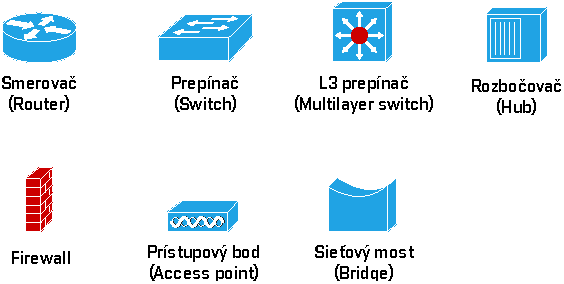
\includegraphics[scale=0.4]{obrazky/net_devices.pdf}
	\end{center}
	\vspace{-5em}
	\caption[Typy sieťových zariadení v lokálnych sieťach]{Typy sieťových zariadení v lokálnych sieťach}
	\label{net-devices}
\end{figure} 

\section{Hierarchický model sietí}
%TODO EDGE
S postupným nárastom sieťových zariadení a komplexnosti siete dochádza v sieťach bez hierarchie k mnohým problémom ako veľké broadcast domény, vysoká cena za port, vysoké zaťaženia zariadení, neprítomnosť redundancie. Preto sa zaviedol hierarchický model siete, ktorý rieši problémy veľkosti a rozsahu broadcast a kolíznych domén, umožňuje efektívne prideľovanie \zkratka{zkIP} adries a oddeľuje zariadenia pracujúce na jednotlivých vrstvách ISO/OSI.  
\\\\
\noindent
Siete sú spravidla delené do 3 vrstiev s definovanými funkciami \cite{Lammle2013}:
\begin{itemize}
	\item Core\,--\,tvorí vysokorýchlostnú chrbticu siete, agreguje dáta z distribučnej vrstvy a mala by byť redundantná. Nároky na rýchlosť portov a výkon zariadenia sú obzvlášť vysoké, a preto sa využívajú prevažne smerovače, ale taktiež ako v distribučnej vrstve dnes už aj L3 prepínače.
	\item Distribučná (Distribution)\,--\,agreguje dáta z prístupovej vrstvy, vytvára a oddeľuje broadcast domény, riadi smerovanie medzi \zkratka{zkVLAN} a  filtrovanie paketov. Táto vrstva kvôli zabezpečeniu dostupnosti využíva agregovanie  a redundanciu liniek. Typicky sa skladá zo smerovačov, no v dnešnej dobe hlavne z L3 prepínačov, keďže tie nie sú finančne také náročné. 
	\item Prístupová (Access)\,--\,vstupný bod do siete, ktorý riadi prístup a politiku pre koncové zariadenia, segmentuje sieť, vytvára a separuje kolízne domény. V neposlednej rade zariaďujú prístup k distribučnej vrstve. Je tvorená zariadeniami ako prepínač, rozbočovač alebo prístupový bod.
\end{itemize} 

\begin{figure}[H]
	\begin{center}
		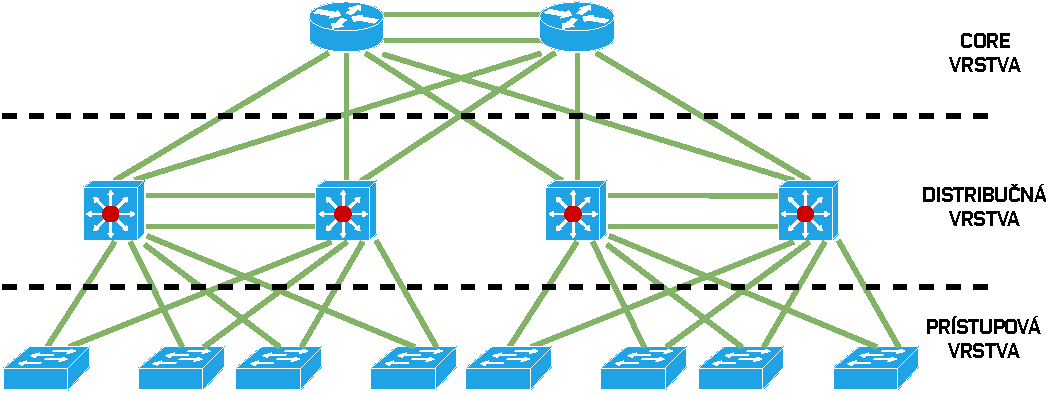
\includegraphics[scale=0.58]{obrazky/hierarchy_network.pdf}
	\end{center}
	\vspace{-11em}
	\caption[Hierarchické rozdelenie siete na vrstvy]{Hierarchické rozdelenie siete na vrstvy}
	\label{net-devices}
\end{figure} 

\noindent
\vspace{2em}
V menších sieťach prevažne malých firiem sa využíva zlučovanie vrstiev nazývaných ako collapsed core, ktoré zlučujú distribučnú a core vrstvu, prípadne zlučujú všetky tri vrstvy dokopy. 

Cieľom hierarchického modelu a dobre navrhnutej siete je dosiahnutie nasledujúcich vlastností:

\begin{itemize}
	\item Škálovateľnosť\,--\,jednoduché a bezproblémové pridanie zariadenia pri raste a rozširovaní siete.
	\item Redundancia\,--\,zabezpečenie vysokej dostupnosti viacnásobnými linkami medzi zariadeniami a zálohovanie samotných zariadení ich redundanciou.
	\item Výkonnosť\,--\,agregovanie liniek a výber dostatočne výkonných zariadení
	\item Bezpečnosť\,--\,zabezpečenie siete na viacerých úrovniach ako napríklad portoch, oddelením segmentov pomocou VLAN, riadením prístupu, šifrovaním a pod.
	\item Manažovateľnosť\,--\,vytvorenie šablón, definovaných štandardov a pravidiel na zaistenie konzistentnosti konfigurácií zariadení na jednoduchšie odhaľovanie chýb. 
	\item Udržovateľnosť\,--\,schopnosť systému prechádzať zmenami komponentov, služieb a vlastností.
\end{itemize}



\section{Úrovne sieťových prvkov}
Sieťové prvky sú zodpovedné nielen za preposielanie dát medzi koncovými stanicami, ale aj za mnohé riadiace dáta medzi sebou, bez ktorých by sieť nebola funkčná. Preto sa jednotlivé protokoly a služby rozdeľujú troch rovín alebo úrovní, a to management, control a data plane. Tieto pojmy sa využívajú vo väčšej miere v softvérovo definovaných sieťach, no sú platné aj v klasickej koncepcii.
 
Úroveň management plane je zodpovedná za konfiguráciu zariadení a riadenie prístupu ku konfiguráciám. Typickými príkladmi protokolov pracujúcich na tejto úrovni sú \zkratka{zkSNMP}, \zkratka{zkAAA}, Syslog, \zkratka{zkSSH} a mnohé ďalšie \cite{Singh2018}. Druhá úroveň, control plane má na starosti prevažne smerovanie, teda kadiaľ budú pakety smerované a prenáša riadiace a signalizačné informácie pre protokoly ako napríklad, \zkratka{zkOSPF}, Spanning tree, \zk{zkFHRP} \cite{Singh2018}. Poslednou úrovňou je data plane nazývaná často aj forwarding plane, ktorá prepína pakety na daný port na základe rozhodnutie z control plane. Táto časť sieťových prvkov musí byť veľmi rýchla, aby zaistila nízku odozvu a dostatočne vysoké prenosové rýchlosti. Nižšie uvedený obrázok \ref{sdn-planes} reflektuje tok dát z jednej úrovne do druhej a tiež medzi dvoma susednými zariadeniami. Úroveň management plane zodpovedná za konfiguráciu zariadenia a nastavuje úroveň control plane, v tomto prípade smerovanie z zariadení. Po výmene informácií so susednými smerovačmi sa vytvoria príslušné tabuľky a nakoniec smerovacia tabuľka, ktorá sa využíva pri rozhodovaní prepínania paketov v úrovni data plane.

\begin{figure}[H]
	\begin{center}
		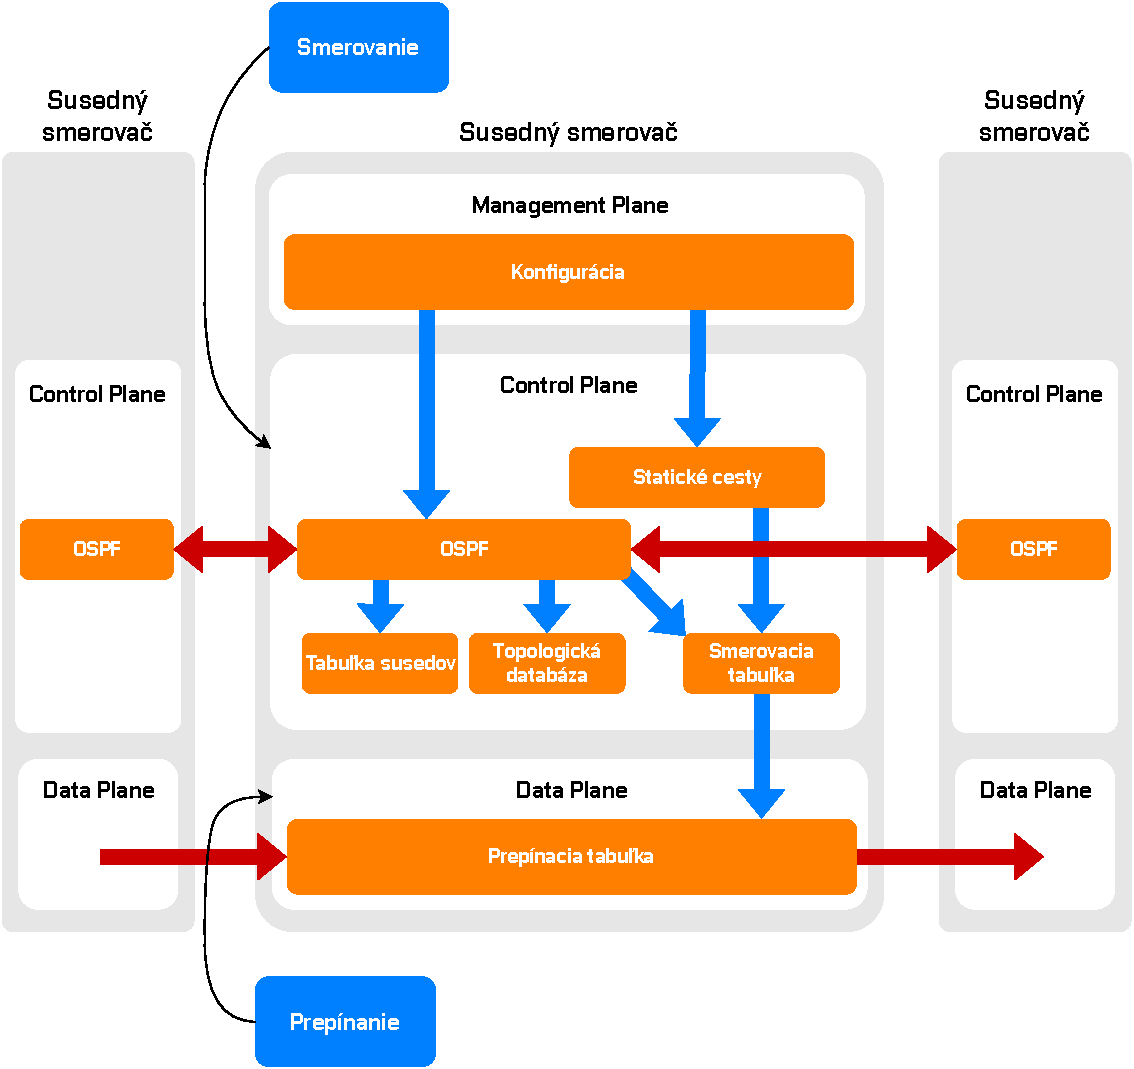
\includegraphics[scale=0.6]{obrazky/SDN_planes.pdf}
	\end{center}
	\caption[Rozdelenie úrovní v smerovači, tok informácií v jeho vnútri a medzi susednými smerovačmi]{Rozdelenie úrovní v smerovači, tok informácií v jeho vnútri a medzi susednými smerovačmi \cite{Pepelnjak2013}}
	\label{sdn-planes}
\end{figure} 


%TODO 3 za tried source interfaces


\section{Riadenie a zneužitie prístup}
AAA, username, accounts, enable psswd, ssh, ACL(data plane, je to data plane?) 92, 111, 112, bannery plus logovanie neuspesnych pristupov

\section{Smerovacie protokoly}
autentizacia, passive, ip source routing, urpf


\section{Identifikácia zariadení, pravidiel a nastavení}
host,domainname, acl remark, int description, vlan description

\section{Šifrovanie hesiel}

\section{Logovanie}
syslog, snmp nastavenie oboch, plus co logovat, teda accouting a logovanie deny pravidiel, 93

\section{Synchronizácia času}
ntp + amplifikacne utoky

\section{Záloha a zabezpečenie konfigurácií}
archive, tftp, scp, delete protection, logovanie zmien, mozno netreba, ak je AAA accounting
\section{Správanie pri vysokom zaťažení}
68-71, storm control
\section{Monitorovanie výkonu siete}
SPAN NETFLOW
\section{Problémy vrstvy L2}
access, max, hopping, double tagging, blackhole, default access a trunk, dtp, spanning tree, dot1x, vtp
\section{First Hop Security}
130 - 138 140 144-148 aj mac spoof a mac floof, teda spanning tree prikazy!!!
http://isp-servis.com/?p=191
\section{First Hop Redundancy Protocols}

\section{Tunely}
\section{Mapovanie siete a objavovanie zariadení}
proxy arp, 88-91, lldp, cdp, 139
\section{Nepoužívané a nebezpečné služby}
\section{Ostatné}
source interfaces
loopback
shutdown 

%% Vložení souboru 'text/navrh.tex' s úvodem
\chapter{Návrh}
\phantomsection

TODO\\
Excel tabuľka s redukciou stĺpcov(checklist) - možno do príloh, ak to bude rozsiahle\\
Checklist ako vznikal a ako boli vypĺňaná polia severity a facility\\
Rozdelenie príkazov\\
Rozdelenie zariadení podľa vrstvy - popísať\\
Stromová štruktúra a koncept fungovania\\
Možno fungovanie cez nejaký UML diagram (sekvenčný?)\\
Prečo konfigurák YAML, výhody a porovnanie s JSON a XML\\
Niečo o Pythone a prečo bol vybraný (možno do implementácie)\\
Popísať konfiguračné súbory device.yaml module.yaml (možno do implementácie)\\


%% Vložení souboru 'text/implementacia.tex' s úvodem
\chapter{Implementácia}
\phantomsection

\section{Použité technológie}
 \subsection{Python}
 Python \cite{B4mfUgNUpPnXbiEr} je objektovo orientovaný, interpretovaný programovací jazyk vytvorený holanďanom Guidom van Rossom. Radí sa k vysokoúrovňovým programovacím jazykom a umožňuje automatickú správu pamäte, teda programátor nie je nútený explicitne potrebnú pamäť alokovať a uvolňovať. Jeho výhodou je práve fakt, že je interpretovaný a teda programy napísané v ňom nemusia byť preložené pre danú platformu, ale postačuje spustenie zdrojového kódu pomocou interpretu nainštalovaného na danom systéme. Interpret jazyka Python je dostupný pre Microsoft Windows, GNU/Linux, macOS a mnoho ďalších vstavaných a exotickejších systémov. Syntax jazyku Python je založená na syntaxi jazyku C, no zdrojový kód je čitateľnejší a na vymedzenie funkčných blokov využíva odsadenie, vďaka čomu je kód čitateľnejší. V súčasnosti sa využíva syntax a interpret dvoch verzií, a to verzie 2.x a 3.x, ktoré sú vzájomne nekompatibilné, z dôvodu rozdielnych syntaktických konštrukcií. Prvá zo zmienených verzií však čoskoro prestane byť podporovaná. Z tohto dôvodu je vhodnejšie použiť na novo vyvíjané programy verziu 3.x. Prednosťou je 
  
 Práve pre vyššie zmienené výhody a to najmä dobrú čitateľnosť kódu, rozšíriteľnosť  medzi programátormi, ako aj spustenie na rôznych platformách bol Python zvolený za programovací jazyk pre túto diplomovú prácu.
 \subsection{YAML}
 YAML \cite{Jd4UTaVyTULvXDoN} je jazyk na serializáciu dát vo forme veľmi dobre čitateľnej pre človeka. Bol inšpirovaný konceptami a syntaxou jazykov C a Python. Dovoľuje definovať primitíva z týchto programovacích jazykov ako zoznamy, asociatívne polia, reťazce a zároveň v jednom súbore dovoľuje definovať viac dokumentov.
 
 Pre konfiguračné súbory boli spočiatku uvažované tri metódy. Prvou možnosťou na serializáciu dát bol jazyk XML, tento formát však nie je tak dobre čitateľný pre človeka a je tu väčšia pravdepodobnosť zanesenia chýb z dôvodu uzatvárania značiek. Druhou možnosťou bolo využitie syntaxe jazyka JSON, no problémom je, že nepodporuje vkladanie komentárov, preto nie je vhodný na konfiguračné súbory. Poslednou možnosťou bolo vytvorenie vlastnej syntaxi a vlastného analyzátoru, to je však pre potreby diplomovej práce zbytočné a hotové riešenie v podobe YAML je dostatočné a eliminuje všetky nedostatky vyššie zmienených jazykov určených na serializáciu dát. Použitý jazyk Python naviac disponuje viacerými knižnicami na prácu s jazykom YAML.  
 \newpage
 \subsection{Regulárne výrazy}
 %nejaký obkec okolo (krátko), prečo sú vhodné, ako budú použité
 Regulárnym výrazom sa rozumie sekvencia znakov, ktorá definuje určitý vzor \cite{sBBUt3Q3bPUfAMue}. Často sa namiesto dlhého názvu využíva skratka ``regex``. Regulárne výrazy sa používajú na vyhľadávanie alebo výmenu reťazcov v texte pričom na to využívajú znaky s vopred definovanou sémantikou. V diplomovej práci budú použité na vyhľadávanie prítomnosti alebo absencii nastavení v konfigurácií zariadení. 

\section{Konfiguračné súbory}
%možno do implementácie, automaticke zistovaine niektorych atributov
\subsection{Súbor popisujúci zariadenie}
\begin{lstlisting}[frame=single,numbers=right,caption={Konfiguračný súbor device.yaml ktorý popisuje základné informácie o jednom konkrétnom zariadení},label=lst:lldp,basicstyle=\ttfamily\small, keywordstyle=\color{black},language=python,breaklines=true]
---
# Hostname of device
hostname: "sw1-access"

# Path to configuration file of device
config: "sw1_access-config.txt"

# Version of running operating system
version: "12.2(55)SE12"

# L3 protocols which are used 
# not only available but literally used and enabled
l3_protocols:
- "ipv4"
- "ipv6"

# Manufacturer of device
# Same directory name has to be created inside 
# directory "Modules", where all modules 
# for this vendor are stored
vendor: "cisco"

# Operating system
os: "ios"

# Type of device
# Types: [r(router), l3sw(L3 switch), l2sw(L2 switch)]
facility: "l3sw"

# Type of layer where facility is installed
# Types: [core/edge, distribution, access, collapsed all, 
# collapsed distribution access, 
# collapsed core distribution]
facility-layer: "access"

# Exclude modules which are specified in file 
# "modules_by_facility.yaml" for specific 
# "facility-layer" you do not want to be used
excluded-modules:
- "dot1x.py"

# Include modules which are not 
# part of  specific "facility-layer"
# in file "modules_by_facility.yaml" 
# and you want to use them.
include-modules: 
- "cdp.py"
- "portsec-max-mac.py"

# All available interfaces, roles of interfaces
# can be specified, roles such as "access" or "trunk"
# are assigned automatically according to config 
# and more than one type can be assigned to port
# Roles: [access, trunk, wan, toinet, access-datacenter,
# wlan, to_distribution_layer, to_core_layer, unused, none]   
interfaces:
- FastEthernet 0/1: "access"
- FastEthernet 0/2: "access-datacenter"
- FastEthernet 0/3: "access"
- FastEthernet 0/4: 
- "trunk"
- "to-core-layer"

# SHA1 hash of input configuration of device
input-config-hash: "12975910C3E6352B5B2BDEE81FA2FC4653A5BD59"

# SHA1 hash of current fix configuration 
fix-hash: "86F7E437FAA5A7FCE15D1DDCB9EAEAEA377667B8"

\end{lstlisting}

\subsection{Súbor popisujúci modul}

\begin{lstlisting}[frame=single,numbers=right,caption={Konfiguračný súbor cdp\_module.yaml ktorý pobsahuje informácie na nájdenie problému, jeho odstránenie a informácie do správy},label=lst:lldp,basicstyle=\ttfamily\small, keywordstyle=\color{black},language=python,breaklines=true]
---
# Module name, it will be seen in report output
name: "CDP disabled"

# Instance name or identifier, e.g. OSPF processes are used
instance-name: ""

# Type of configuration command
# Types: [o, i, m, b]
# o - one time in config e.g. "ip ssh version 2"
# i - applied on interface (onetime/manytime) e.g. portsecurity, ACL
# m - multiple time e.g. password for telnet, password for eigrp processes
# b - both interface and general e.g. CDP, root guard
type: "b"

# Type of device
# Types: [r(router), l3sw(L3 switch), l2sw(L2 switch), all]
default-facility: "all"

# Type of layer where facility is installed
# Types: [core/edge, distribution, access, collapsed all, collapsed distribution access, collapsed core distribution, all]
default-facility-layer: "all"

# Run only when module(s) below have found an error
# means security problem or missing configuration
run-if-error-returned: 
- "none"

# Run only when module(s) below have not find an error
# means configuration which module(s) looking for is present
run-if-error-returned: 
- "none"

# Variables needed for generating configuration fix
# e.g. - snmp-user: "administrator1"
instance-public-vars:
- "none"

# Variable that holds secret until configuration fix is generated
# after that it is cleared due to security
# e.g. - password: "" 
instance-secret-vars:
- "none"

#------------------------------------------------------------
# GENERAL CMD CONFIG
#------------------------------------------------------------
name-cmd-general: "CDP Globally DISABLED"

# Severity which defines importance of found problem 
# Types: [critical, high, medium, low, notice]
default-cmd-general-severity: "critical"

# Severity which defines importance of found problem 
# Types: [critical, high, medium, low, notice]
# Default: none
user-cmd-general-severity: "none"

#Regex to match and find occurrence
regex-cmd-general: "no cdp run"

# Specifies whether module should look for regex occurrence
# or non-occurrence match
# Types:
# occurrence - set when regex occurrence in variable "regex-cmd-general" signalize no issue
# nonoccurrence - set when regex non-occurrence in variable "regex-cmd-general" signalize no issue
regex-cmd-general-occurrence: "occurrence"

# Boolean variable to store whether regex matches or not 
regex-cmd-general-match-status: "False"

# Command to resolve problem
# String when one line command, for multiple command setup a list
fix-cmd-general: "no cdp run"

# Notice seen in report when fix will be applied
# e.g. notice about something can stop working after applying fix
fix-cmd-general-notice: "Fix may cause CISCO IP telephony malfunction"

# Boolean which indicates whether a fix will be ignored or applied
fix-cmd-general-ignore: "True"

# Comment to specify reason why command for fix is ignored,
# reason or comment about accepting the risk
fix-cmd-general-ignore-comment: "Enabled due to CISCO IP Telephony"

# Boolean which indicates finding an issue is false positive
fix-cmd-general-false-positive: "False"

# Comment to specify reason why is finding marked as false positive
fix-cmd-general-false-positive-comment: "none"

#------------------------------------------------------------
# INTERFACE CMD CONFIG
#------------------------------------------------------------
name-cmd-affected-ports: "CDP on interface DISABLED"

# Severity which defines importance of found problem on affected interface
# Types: [critical, high, medium, low, notice]
default-cmd-affected-ports-severity: "critical"

# Severity which defines importance of found problem on affected interface
# Types: [critical, high, medium, low, notice]
# Default: none
user-cmd-affected-ports-severity: "none"

#Regex to match and find occurrence
regex-cmd-affected-ports: "no cdp enable"

# Specifies whether module should look for regex occurrence
# or non-occurrence match
# Types:
# occurrence - set when regex occurrence in variable "regex-cmd-general" signalize no issue
# nonoccurrence - set when regex non-occurrence in variable "regex-cmd-general" signalize no issue
regex-cmd-affected-ports-occurrence: "occurrence"

# Boolean variable to store whether regex matches or not on interfaces 
regex-cmd-affected-ports-match-status: "False"

# List of ports where issue is found when variable "type" is "i" or "b"
affected-ports:
- FastEthernet 0/1
- FastEthernet 0/2

# Command to resolve problem on interfaces
# String when one line command, for multiple command setup a list
fix-cmd-affected-ports: "no cdp enable"

# Notice seen in report when fix will be applied on affected interface
# e.g. notice about something can stop working after applying fix
fix-cmd-affected-ports-notice: "Fix may cause CISCO IP telephony malfunction"

# Boolean which indicates whether a fix will be ignored or applied
fix-cmd-affected-ports-ignore: "True"

# Comment to specify reason why command for fix is ignored
fix-cmd-affected-ports-ignore-comment: "Enabled due to CISCO IP Telephony"

# Boolean which indicates finding an issue is false positive
fix-cmd-affected-ports-false-positive: "False"

# Comment to specify reason why is finding marked as false positive
fix-cmd-affected-ports-positive-comment: "none"


#------------------------------------------------------------
# INTERFACE CMD IGNORE CONFIG
#------------------------------------------------------------

name-cmd-explicit-ignored-ports: "CDP running on interfaces IGNORED"

# Severity which defines importance of found problem on affected interface
# Types: [critical, high, medium, low, notice]
default-cmd-explicit-ignored-ports-severity: "critical"

# Severity which defines importance of found problem on affected interface
# Types: [critical, high, medium, low, notice]
# Default: none
user-cmd-explicit-ignored-ports-severity: "none"

# List of ports which should be ignored when "type" is "i" or "b"
explicit-ignored-ports:
- FastEthernet 0/3
- FastEthernet 0/4

# Command to resolve problem on interfaces which are ignored
# Can be blank when you want just ignore ports, some commands
# like CDP can have on ignored ports command "cdp enable" when
# globally is disabled
fix-cmd-explicit-ignored-ports: "cdp enable"

# Notice seen in report when fix will be applied on ignored interface
# e.g. notice about something can stop working after applying fix
fix-cmd-explicit-ignored-ports-notice: "Enabling CDP on interface(s) can lead to serious attacks"

# Comment to specify reason why ignore command is applied
fix-cmd-explicit-ignored-ports-comment: "Enabled due to CISCO IP Telephony"

\end{lstlisting}

%\section{Moduly}




%% Vložení souboru 'text/zaver' se závěrem
\chapter*{Záver}
\phantomsection
\addcontentsline{toc}{chapter}{Záver}


%Buducnost - oznacovanie flase possive + komenty\\
%Dorobit backend - server \\
%co som mal spravit
%co som spravilk

% co sa nepodarili
% v skratke vyhody
% co bolo nutne nastudovat plus z kolko guidov som cerpal





Cieľom tejto diplomovej práce bol návrh a následná implementácia programu na nájdenie bezpečnostných a prevádzkových nedostatkov v sieťových zariadeniach, ako aj ich náprava pomocou generovania opravnej konfigurácie. Z tohto dôvodu bola naštudovaná problematika bezpečnosti a prevádzky sieťových zariadení a ich správna konfigurácia. Z množstva dostupnej literatúry, štandardov a odporúčaní bol vytvorený zoznam odporúčaní, na základe ktorého boli zostavované YAML moduly pre výsledný program. Tento zoznam odporúčaní bol rozšírený aj o hodnotenie závažnosti nedostatkov a priradenie prvkov zoznamu k relevantným zariadeniam v hierarchickom modely siete. Jedná sa teda o unikátne riešenie medzi bezplatnými zoznamami odporúčaní. Tento zoznam môže byť použitý aj na rozšírenie programu o podporu iných výrobcov, ale aj separátne bez akéhokoľvek využitia v programe. Vzhľadom na časovú náročnosť boli vytvorené moduly zatiaľ pre zariadenia značky Cisco. Bolo nutné zanalyzovať niekoľko stovák príkazov a ich povolených kombinácií, vytvoriť pre ne korešpondujúce regulárne výrazy a následne vytvoriť viac ako 220 YAML modulov zodpovedných za nájdenie problémov v konfiguráciách. 

Ako implementačný jazyk bol využitý Python 3.7, ktorý zaisťuje prenositeľnosť programu na viaceré platformy. Program na rozdiel od konkurencie umožňuje rozšírenie vďaka modularite aj na ďalších výrobcov sieťových zariadení a pridáva kontrolu aj pre topológie využívajúce IPv6. Taktiež rešpektuje hierarchický model siete, a teda generuje oveľa menej falošne pozitívnych správ, keďže kontroluje iba nastavenia typické pre danú vrstvu, na ktorej zariadenie operuje. Jeho výstupom je okrem iného aj prehľadná správa o kontrole zobraziteľná v PDF alebo vo webovom prehliadači. Naviac ako jediný z porovnávaných bezplatných riešení umožňuje automatické vygenerovanie nápravy, pokiaľ je to z charakteru príkazu možné. 

Napriek rôznym komplikáciám, a to hlavne neposkytnutie konfigurácií z reálnych sietí, ktoré boli vopred dohodnuté, prebehlo aj testovanie pomocou vyexportovaných konfigurácií z topológií vytvorených v nástroji GNS3.

Z pôvodného návrhu sa nepodarilo vzhľadom na časovú náročnosť celého programu implementovať vyhľadávanie zoznamu útokov a problémov aktuálne bežiacej verzie operačného systému, no počíta sa s implementáciou tejto funkcionality v budúcnosti. Ďalším rozšírením, ktoré je možné aplikovať, je pridanie podpory na ďalších výrobcov ako Juniper a HP. Využiteľné by bolo taktiež možnosť editovať záverečné správy pridaním back-endu pre HTML správy.


%% Vložení souboru 'text/literatura' se seznamem literatury\\
% Pro sazbu seznamu literatury použijte jednu z následujících možností

%%%%%%%%%%%%%%%%%%%%%%%%%%%%%%%%%%%%%%%%%%%%%%%%%%%%%%%%%%%%%%%%%%%%%%%%%
%1) Seznam citací definovaný přímo pomocí prostředí literatura / thebibliography

\begin{literatura}{99}
\bibitem{Milkovich3122018}
MILKOVICH, Devon. 13 Alarming Cyber Security Facts and Stats. In: \textit{Cybint} [online]. 3.12.2018 [cit. 2019-11-08]. Dostupné z: https://www.cybintsolutions.com/cyber-security-facts-stats/

\bibitem{Vyncke2008}
VYNCKE, Eric a Christopher PAGGEN. \textit{LAN switch security: What hackers know about your switches}. Indianapolis, IN: Cisco Press, 2008. ISBN :978-1-58705-256-9.	
	
\bibitem{McMillan2018}
MCMILLAN, Troy. \textit{CCNA security study guide: exam 210-260}. Indianapolis, Indiana: Sybex, a Wiley Brand, 2018. ISBN 978-111-9409-939.
	
\bibitem{Stallings2011}
STALLINGS, William. \textit{Network security essentials: applications and standards}. 4th ed. Boston: Prentice Hall, 2011. ISBN 978-0-13-610805-4.

\bibitem{Jackson2010}
JACKSON, Chris. \textit{Network security auditing}. Indianapolis, IN: Cisco Press, 2010. Cisco Press networking technology series. ISBN 978-1-58705-352-8.

\bibitem{7TVhmfuQFbsOANAz}
Guide for Conducting Risk Assessments: NIST Special Publication 800-30. In: \textit{NIST} [online]. 2012 [cit. 2019-11-08]. Dostupné z: https://nvlpubs.nist.g\
ov/nistpubs/Legacy/SP/nistspecialpublication800-30r1.pdf

	
	
	
\bibitem{Alsadeh1252015}
ALSADEH, Ahmad. Augmented SEND: Aligning Security, Privacy, and Usability. In: \textit{RIPE NCC} [online]. 12.5.2015 [cit. 2019-11-02]. Dostupné z: https://ripe70.ripe.net/presentations/67-RIPE70-SEND.pdf
\bibitem{Podermanski1222015}
PODERMAŃSKI, Tomáš a Matěj GRÉGR. Bezpečné IPv6: zkrocení zlých směrovačů. In: \textit{ROOT.CZ} [online]. 12.2.2015 [cit. 2019-11-02]. Dostupné z: https://www.root.cz/clanky/bezpecne-ipv6-zkroceni-zlych-smerovacu/
\bibitem{Khandelwal2016}
KHANDELWAL, Manjul. OSPF Security: Attacks and Defenses. In: \textit{SANOG} [online]. 2016 [cit. 2019-11-04]. Dostupné z: https://www.sanog.org/resources/sanog28/SANOG28-Tutorial\_OSPF-Security-Attacks-and-Defences-Manjul.pdf
\bibitem{Podermanski1932015}
PODERMAŃSKI, Tomáš a Matěj GRÉGR. Bezpečné IPv6: když dojde keš --- obrana. In: \textit{ROOT.CZ} [online]. 19.3.2015 [cit. 2019-11-02]. Dostupné z: https://www.root.cz/clanky/bezpecne-ipv6-kdyz-dojde-kes-obrana/
\bibitem{Podermanski1232015}
PODERMAŃSKI, Tomáš a Matěj GRÉGR. Bezpečné IPv6: když dojde keš. In: \textit{ROOT.CZ} [online]. 12.3.2015 [cit. 2019-11-02]. Dostupné z: https://www.root.cz/clanky/bezpecne-ipv6-kdyz-dojde-kes/
\bibitem{Podermanski532015}
PODERMAŃSKI, Tomáš a Matěj GRÉGR. Bezpečné IPv6: trable s multicastem. In: \textit{ROOT.CZ} [online]. 5.3.2015 [cit. 2019-11-02]. Dostupné z: https://www.root.cz/clanky/bezpecne-ipv6-trable-s-multicastem/
\bibitem{Gregr2622015}
GRÉGR, Matěj a Tomáš PODERMAŃSKI. Bezpečné IPv6: vícehlavý útočník. In: \textit{ROOT.CZ} [online]. 26.2.2015 [cit. 2019-11-02]. Dostupné z: https://www.root.cz/clanky/bezpecne-ipv6-vicehlavy-utocnik/
\bibitem{Podermanski1922015}
PODERMAŃSKI, Tomáš a Matěj GRÉGR. Bezpečné IPv6: trable s hlavičkami. In: \textit{ROOT.CZ} [online]. 19.2.2015 [cit. 2019-11-02]. Dostupné z: https://www.root.cz/clanky/bezpecne-ipv6-trable-s-hlavickami/
\bibitem{Gregr522015}
GRÉGR, Matěj a Tomáš PODERMAŃSKI. Bezpečné IPv6 : směrovač se hlásí. In: \textit{ROOT.CZ} [online]. 5.2.2015 [cit. 2019-11-02]. Dostupné z: https://www.root.cz/clanky/bezpecne-ipv6-smerovac-se-hlasi/
\bibitem{zXCpMaLbN1J7D1z2}
IPv6 First-Hop Security Configuration Guide. In: \textit{Cisco} [online]. San Jose [cit. 2019-11-02]. Dostupné z: https://www.cisco.com/c/en/us/td/docs/ios-xml/ios/ipv6\_fhsec/configuration/15-1sg/ip6f-15-1sg-book.pdf
\bibitem{Bouska2007}
BOUŠKA, Petr. \textit{Cisco IOS 12 - IEEE 802.1x a pokročilejší funkce} [online]. In: . 2007 [cit. 2019-11-02]. Dostupné z: https://www.samuraj-cz.com/clanek/cisco-ios-12-ieee-802-1x-a-pokrocilejsi-funkce/
\bibitem{yDzYjF1hoACahpg1}
MOLENAAR, René. Cisco IOS features that you should disable or restrict. In: \textit{NetworkLessons.com} [online]. [cit. 2019-11-02]. Dostupné z: https://networklessons.com/uncategorized/cisco-ios-features-that-you-should-disable-or-restrict
\bibitem{Bouska2009}
BOUŠKA, Petr. Cisco IOS 23 - Autentizace uživatele na switchi vůči Active Directory. In: \textit{SAMURAJ-cz} [online]. 2009 [cit. 2019-11-02]. Dostupné z: https://www.samuraj-cz.com/clanek/cisco-ios-23-autentizace-uzivatele-na-switchi-vuci-active-directory/
\bibitem{Barker2019}
BARKER, Elaine a Allen ROGINSKY. Transitioning the Use of Cryptographic Algorithms and Key Lengths. In: \textit{NIST} [online]. 2019 [cit. 2019-11-02]. Dostupné z: https://nvlpubs.nist.gov/nistpubs/SpecialPublications/NIST.SP.800-131Ar2.pdf
\bibitem{o31nYG4kn98wWNRS}
VYNCKE, Erik. ND on wireless links and/or with sleeping nodes. In: \textit{IETF} [online]. [cit. 2019-11-02]. Dostupné z: https://www.ietf.org/proceedings/89/slides/slides-89-v6ops-3.pdf
\bibitem{DrTLsgXv24lxeIIM}
CIS Cisco IOS 15 Benchmark. In: \textit{Center For Internet Security} [online]. 2015 [cit. 2019-11-02]. Dostupné z: https://www.cisecurity.org/benchmark/cisco/
\bibitem{Singh2018}
SINGH, Shashank. Cisco Guide to Harden Cisco IOS Devices. In: \textit{Cisco} [online]. 2018 [cit. 2019-11-02]. Dostupné z: https://www.cisco.com/c/en/us/support/docs/ip/access-lists/13608-21.html
\bibitem{Graesser2001}
GRAESSER, Dana. Cisco Router Hardening Step-by-Step. In: \textit{SANS Institute} [online]. 2001 [cit. 2019-11-02]. Dostupné z: https://www.sans.org/reading-room/whitepapers/firewalls/paper/794
\bibitem{Pilihanto2012}
PILIHANTO, Atik. A Complete Guide on IPv6 Attack and Defense. In: \textit{SANS Institute} [online]. SANS Institute, 2012 [cit. 2019-11-02]. Dostupné z: https://www.sans.org/reading-room/whitepapers/detection/paper/33904
\bibitem{Rey2016}
REY, Enno, Antonios ATLASIS a Jayson SALAZAR. MLD Considered Harmful. In: \textit{RIPE NCC} [online]. 2016 [cit. 2019-11-02]. Dostupné z: https://ripe72.ripe.net/presentations/74-ERNW\_RIPE72\_MLD\_Considered\_Harmful\_v1\_light\_web.pdf
\bibitem{Vyncke2012}
VYNCKE, Erik. IPv6 First Hop Security: the IPv6 version of DHCP snooping and dynamic ARP inspection. In: \textit{Slidde Share} [online]. 2012 [cit. 2019-11-02]. Dostupné z: https://www.slideshare.net/IKTNorge/eric-vyncke-layer2-security-ipv6-norway
\bibitem{77Eg8gGc0CKWfGBi}
IPv6 First-Hop Security Configuration Guide. In: \textit{Cisco} [online]. 2012 [cit. 2019-11-02]. Dostupné z: https://www.cisco.com/c/en/us/td/docs/ios-xml/ios/ipv6\_fhsec/configuration/15-s/ip6f-15-s-book/ip6-snooping.html
\bibitem{Gregr2011}
GREGR, Matej, Petr MATOUSEK, Miroslav SVEDA a Tomas PODERMANSKI. Practical IPv6 monitoring-challenges and techniques. In: \textit{12th IFIP/IEEE International Symposium on Integrated Network Management (IM 2011) and Workshops}. IEEE, 2011, 2011, s.~650-653. DOI: 10.1109/INM.2011.5990647. ISBN 978-1-4244-9219-0. Dostupné také z: http://ieeexplore.ieee.org/document/5990647/
\bibitem{1xYhFLUJF9lmHMC0}
PODERMAŃSKI, Tomáš a Matějj GRÉGR. \textit{Deploying IPv6 - practical problems from the campus perspective} [online]. In: . [cit. 2019-11-02].
\bibitem{Martin2016}
MARTIN, Tim. IPv6 Sys Admin Style. In: \textit{SlideShare} [online]. 2016 [cit. 2019-11-02]. Dostupné z: https://www.slideshare.net/tjmartin2020/ipv6-sysadmins-63071235
\bibitem{uYLsMtQInofenpV3}
Cisco SAFE Reference Guide. In: \textit{CIsco} [online]. San Jose, CA, 8 Júl 2018 [cit. 2019-11-02]. Dostupné z: https://www.cisco.com/c/en/us/td/docs/solutions/Enterprise/Security/SAFE\_RG/SAFE\_rg.pdf
\bibitem{JnCqiekTXFe2KIyx}
SAFE Overview Guide: Threats, Capabilities, and the Security Reference Architecture. In: \textit{Cisco} [online]. Január 2018 [cit. 2019-11-02]. Dostupné z: https://www.cisco.com/c/dam/en/us/solutions/collateral/enterprise/design-zone-security/safe-overview-guide.pdf

\bibitem{Akin2002}
AKIN, Thomas. \textit{Hardening Cisco routers}. Sebastopol: O'Reilly, 2002. ISBN 05-960-0166-5.

\bibitem{Hucaby2010}
HUCABY, Dave, Steve MCQUERRY, Andrew WHITAKER a Dave HUCABY. \textit{Cisco router configuration handbook}. 2nd ed. Indianapolis, IN: Cisco Press, 2010. ISBN 978-1-58714-116-4.
\bibitem{Satrapa2019}
SATRAPA, Pavel. \textit{IPv6: internetový protokol verze 6}. 4. aktualizované a rozšířené vydání. Praha: CZ.NIC, z.s.p.o., 2019. CZ.NIC. ISBN 978-808-8168-430.



\end{literatura}


%%%%%%%%%%%%%%%%%%%%%%%%%%%%%%%%%%%%%%%%%%%%%%%%%%%%%%%%%%%%%%%%%%%%%%%%%
%%2) Seznam citací pomocí BibTeXu
%% Při použití je nutné v TeXnicCenter ve výstupním profilu aktivovat spouštění BibTeXu po překladu.
%% Definice stylu seznamu
%\bibliographystyle{unsrturl}
%% Pro českou sazbu lze použít styl czechiso.bst ze stránek
%% http://www.fit.vutbr.cz/~martinek/latex/czechiso.tar.gz
%%\bibliographystyle{czechiso}
%% Vložení souboru se seznamem citací
%\bibliography{text/literatura}
%
%% Následující příkaz je pouze pro ukázku sazby literatury při použití BibTeXu.
%% Způsobí citaci všech zdrojů v souboru odkazy.bib, i když nejsou citovány v textu.
%\nocite{*}
%\bibliographystyle{slovakiso}
%\bibliography{text/literatura}
%\nocite{*}

%% Vložení souboru 'text/zkratky' se seznam použitých symbolů, veličin a zkratek
\begin{seznamzkratek}{KolkokMiesta}

	\novazkratka{zkCIA} % název
		{CIA} % zkratka
		{confidentiality, integrity, availability -- dôvernosť, integrita, dostupnosť} % rozvinutí zkratky

	\novazkratka{zkDDoS} % název
		{DDoS} % zkratka
		{Distributed Denial of Service -- distribuované odoprenie služby} %rozvinutí zkratky
	
	\novazkratka{zkDoS} % název
	{DoS} % zkratka
	{Denial of Service -- odoprenie služby} %rozvinutí zkratky

	\novazkratka{zkACL} % název
		{ACL} % zkratka
		{Access Control List -- zoznam pre riadenie prístupu} %rozvinutí zkratky

	\novazkratka{zkCVSS} % název
		{CVSS} % zkratka
		{Common Vulnerability Scoring System} %rozvinutí zkratky
		
	\novazkratka{zkIDS} % název
		{IDS} % zkratka
		{Intrusion Detection System -- systém detekcie narušenia} %rozvinutí zkratky

	\novazkratka{zkIPS} % název
		{IPS} % zkratka
		{Intrusion Prevention System -- systém prevencie prienikov} %rozvinutí zkratky

	\novazkratka{zkFHRP} % název
		{FHRP} % zkratka
		{First Hop Redundancy Protocol} %rozvinutí zkratky

	\novazkratka{zkSNMP} % název
		{SNMP} % zkratka
		{Simple Network Management Protocol} %rozvinutí zkratky	
	
	\novazkratka{zkAAA} % název
	{AAA} % zkratka
	{Authentication Authorization Accounting} %rozvinutí zkratky
	
	\novazkratka{zkSSH} % název
	{SSH} % zkratka
	{Secure Shel} %rozvinutí zkratky
	
	\novazkratka{zkOSPF} % název
	{OSPF} % zkratka
	{Open Shortest Path First} %rozvinutí zkratky			

	\novazkratka{zkLAN} % název
	{LAN} % zkratka
	{Local Area Network} %rozvinutí zkratky	

	\novazkratka{zkIP} % název
	{IP} % zkratka
	{Internet Protocol} %rozvinutí zkratky
	
	\novazkratka{zkVLAN} % název
	{VLAN} % zkratka
	{Virtual LAN} %rozvinutí zkratky
	
	\novazkratka{zkARP} % název
	{ARP} % zkratka
	{Address Resolution Protocol} %rozvinutí zkratky

	\novazkratka{zkMAC} % název
	{MAC} % zkratka
	{Media Access Control} %rozvinutí zkratky
	
	\novazkratka{zkLLDP} % název
	{LLDP} % zkratka
	{Link Layer Discovery Protocol} %rozvinutí zkratky

	\novazkratka{zkAPI} % název
	{API} % zkratka
	{Application programming interface} %rozvinutí zkratky
	
	\novazkratka{zkGUI} % název
	{GUI} % zkratka
	{graphical user interface -- grafické užívateľské rozhranie} %rozvinutí zkratky
	


\end{seznamzkratek}


%% Začátek příloh
\prilohy

%% Vysázení seznamu příloh
\seznampriloh

%% Vložení souboru 'text/prilohy' s přílohami
\newgeometry{left=2.5cm,bottom=3.4cm, top=2.5cm}
\chapter{Kontrolný zoznam odporúčaní pre zariadenia CISCO}
\label{apendix:cisco_cmd}

\scriptsize

\begin{longtable}[!htbp]{|L{10em}L{10em}>{\fontfamily{qcr}\selectfont}L{34em}|}
	\caption{Rozpracovaná tabuľka s príkazmi na konfiguráciu zariadení od spoločnosti Cisco}
	\label{tab:cisco_table}\\ \hline
	\centering 
	
	\centering{\hspace{-3em}\vspace{1em}Útok / Problém} & Mitigácia / Nastavenie&{\fontfamily{lmr}\selectfont Príkazy}\\ \hhline{===}
	\endfirsthead
	
	
	\hline
	\centering 
	\centering{\hspace{-3em}Útok / Problém} & Mitigácia / Nastavenie&{\fontfamily{lmr}\selectfont Príkazy}\\ \hhline{===}
	\endhead
	
	
	
	\rowcolor[rgb]{ .97,  .97,  .97} Nemožná identifikácia zariadenia	&Vytvoriť hostname	&hostname $<$hostname$>$\\
	Nemožnosť vzdialeného prístupu	&Vytvoriť doménové meno	&ip domain-name $<$domain$>$\\
	
	\rowcolor[rgb]{ .97,  .97,  .97} Nepovolený prístup k manažovaniu zariadenia	&Vytvoriť a aplikovať ACL pre OOB, Telnet, SSH a pod. a zaznamenať v logu prístupy	&ip access-list standard $<$acl name$>$
	
	\hspace{0.5em}remark permit specifi ip and log
	
	\hspace{0.5em}permit $<$ip address$>$ $<$mask$>$ log-input
	
	\hspace{0.5em}remark deny other and log
	
	\hspace{0.5em}deny any log-input
	
	\vspace{0.5em}
	
	ipv6 access-list $<$acl name$>$
	
	\hspace{0.5em}remark permit specifi ip and log
	
	\hspace{0.5em}permit $<$ipv6 address$>$/$<$prefix$>$ any log-input
	
	\hspace{0.5em}remark deny other and log
	
	\hspace{0.5em}deny any any log-input
	
	\vspace{0.5em}
	{\fontfamily{lmr}\selectfont alebo v global config }
	\vspace{0.5em}
	
	login on-failure log-input
	
	login on-failure trap
	
	login on-failure
	
	login on-success log-input
	
	login on-success trap
	
	login on-success\\
	
	
	
	
	Nepovolený prístup k manažovaniu zariadenia	&Vytvoriť a aplikovať ACL pre Telnet, SSH a pod. a zaznamenať v logu prístupy	&line vty $<$num$>$ $<$num$>$
	
	\hspace{0.5em}ip access-class $<$acl name$>$ in
	
	\hspace{0.5em}ipv6 access-class $<$acl name$>$ in
	
	\vspace{0.5em}line tty $<$num$>$ $<$num$>$
	
	\hspace{0.5em}ip access-class $<$acl name$>$ in
	
	\hspace{0.5em}ipv6 access-class $<$acl name$>$ in\\
	
	
	
	
	
	\rowcolor[rgb]{ .97,  .97,  .97}Neautorizovaný prístup cez nepoužívané a nezabezpečené protokoly na manažment zariadení	&Vypnúť nepoužívané protokoly na prístup k manažovaniu zariadení (telnet a pod.)	&line aux 0
	
	\hspace{0.5em}no exec
	
	\hspace{0.5em}transport input none\\
	
	
	
	
	Prístup bez požadovaných prístupových údajov	&Nakonfigurovanie protokolov na manažment zariadení, aby požadovali prístupové údaje (telnet a pod.)	&line vty $<$num$>$ $<$num$>$
	\hspace{0.5em}password
	
	\hspace{0.5em}login | login local
	
	\vspace{0.5em}line tty $<$num$>$ $<$num$>$
	
	\hspace{0.5em}password
	
	\hspace{0.5em}login | login local
	
	\vspace{0.5em}
	line con $<$num$>$
	
	\hspace{0.5em}password
	
	\hspace{0.5em}login | login local
	
	\vspace{0.5em}line aux $<$num$>$
	
	\hspace{0.5em}password
	
	\hspace{0.5em}login | login local\\
	
	
	
	
	\rowcolor[rgb]{ .97,  .97,  .97}Nepoužívanie zabezpečeného protokolu na manažment zariadení môže viesť k odposluchu	&Zapnutie SSH	&line vty $<$num$>$ $<$num$>$
	
	\hspace{0.5em}login local
	
	\hspace{0.5em}transport input ssh\\
	
	
	
	Nebezpečná verzia 1 protokolu SSH	&SSH verzia 2	&ip ssh version 2\\
	
	
	
	
	\rowcolor[rgb]{ .97,  .97,  .97}Dlhé neaktívne sedenie môže byť zneužité alebo aj fyzický prístup útočníka k aktívnemu sedeniu môže viesť k zmene konfigurácie	&SSH čas vypršania sedenia	&ip ssh timeout $<$timeout seconds$>$\\
	
	
	
	
	Útok na krátky RSA kľúč	&Dĺžka RSA kľúča minimálne 2048 bitov	&crypto key generate rsa modulus 2048\\
	
	
	
	
	\rowcolor[rgb]{ .97,  .97,  .97}Hádanie hesla k RSA kľúču	&SSH maximálny počet neúspešných pokusov	&ip 
	ssh authentication-retries $<$max num$>$\\
	
	
	
	
	Útok hrubou silou na zistenie prihlasovacích údajov	&Špecifikovať čas po ktorý nie je možné po N pokusoch sa prihlásiť	&login block-for 60 attempts 3 within 30\\
	
	
	
	
	\rowcolor[rgb]{ .97,  .97,  .97} Prihlásenie na zariadenie nie je možné kvôli zablokovaniu pre príliš veľa neúspešných pokusov	&Povolenie prístupu administrátorovi na základe IP adresy, keď je protokol na manažovanie zariadení nedostupný kvôli DOS útoku	&login quiet-mode access-class $<$acl name$>$\\
	
	
	
	Možné prihlásenie do zariadenia cez telnet keď je prítomné SSH	&Zakázať telnet ak je SSH aktívne	&line vty $<$num$>$ $<$num$>$
	
	\hspace{0.5em}no transport input all
	
	\hspace{0.5em}no transport input telnet
	\vspace{0.5em}
	
	line tty $<$num$>$ $<$num$>$
	
	\hspace{0.5em}no transport input all
	
	\hspace{0.5em}no transport input telnet
	\vspace{0.5em}
	
	line con $<$num$>$
	
	\hspace{0.5em}no transport input all
	
	\hspace{0.5em}no transport input telnet
	\vspace{0.5em}
	
	line aux $<$num$>$
	
	\hspace{0.5em}no transport input all
	
	\hspace{0.5em}no transport input telnet\\
	
	
	
	
	\rowcolor[rgb]{ .97,  .97,  .97} Útočník nie je informovaný o právnych následkoch	&Právne upozornenie pri prístupe k zariadeniu	&banner motd
	
	banner login
	
	banner exec\\
	
	
	
	Dlhé neaktívne sedenie môže byť zneužité alebo aj fyzický prístup útočníka k aktívnemu sedeniu môže viesť k zmene konfigurácie	&Čas vypršania sedenia pre protokol na manažovanie zariadení	&line vty $<$num$>$ $<$num$>$
	
	exec-timeout 5
	\vspace{0.5em}
	
	line tty $<$num$>$ $<$num$>$
	
	\hspace{0.5em}exec-timeout 5
	\vspace{0.5em}
	
	line con $<$num$>$
	
	\hspace{0.5em}exec-timeout 5
	\vspace{0.5em}
	
	line aux $<$num$>$
	
	\hspace{0.5em}exec-timeout 5\\
	
	
	
	
	\rowcolor[rgb]{ .97,  .97,  .97} Možnosť prečítať heslá z uniknutých konfigurácií	&Zašifrovanie hesiel v otvorenej podobe	&service password-encryption\\
	
	
	
	
	Nepovolená zmena konfigurácie zariadenia	&Vytvorenie hesla na editovanie konfigurácie zariadenia	&enable secret $<$secret password$>$\\
	
	
	
	
	\rowcolor[rgb]{ .97,  .97,  .97} Nepovolená zmena konfigurácie zariadenia	&Vytvorenie hesla na editovanie konfigurácie zariadenia	&no enable password $<$password$>$\\
	
	
	
	Nepovolený prístup k manažmentu konfigurácie zariadenia	&Lokálne zabezpečené účty	&username secret $<$username$>$ $<$secret password$>$\\
	
	
	
	\rowcolor[rgb]{ .97,  .97,  .97} Nepovolený prístup k manažmentu konfigurácie zariadenia	&Lokálne zabezpečené účty	&no username password  $<$username$>$ $<$password$>$\\
	
	
	
	Centrálna správa prihlásení a dohľadateľnosť zmien v konfigurácií	&Definovanie a povolenie AAA serveru na prihlásenie a definovanie záložného prihlásenia	&aaa new-model
	
	radius server $<$radius server name$>$
	
	\hspace{0.5em}address ipv4 $<$ip adddress$>$ / address ipv6 $<$ipv6 adddress$>$
	
	\hspace{0.5em}key $<$password$>$
	\vspace{0.5em}
	
	{\fontfamily{lmr}\selectfont alebo}
	
	\vspace{0.5em}
	radius-server host $<$ip adddress$>$
	
	radius-server key $<$password$>$
	
	\vspace{0.5em}
	
	aaa group server radius $<$radius group$>$
	
	\hspace{0.5em}server name $<$radius server name$>$
	
	aaa authentication login default / $<$radius login$>$ group 
	
	\hspace{0.5em}$<$radius group$>$ local enable
	
	line tty $<$num$>$ $<$num$>$
	
	\hspace{0.5em}login authentication default / $<$radius login$>$
	
	line vty $<$num$>$ $<$num$>$
	
	\hspace{0.5em}login authentication default / $<$radius login$>$
	
	line con $<$num$>$
	
	\hspace{0.5em}login authentication default / $<$radius login$>$
	
	line aux $<$num$>$
	
	
	\hspace{0.5em}login authentication default / $<$radius login$>$\\
	
	
	
	
	\rowcolor[rgb]{ .97,  .97,  .97} Centrálna správa prihlásení a dohľadateľnosť zmien v konfigurácií	&Definovanie a povolenie AAA serveru na prihlásenie a definovanie záložného prihlásenia	&aaa new-model
	
	tacacs server $<$tacacs server name$>$
	
	\hspace{0.5em}address ipv4 $<$ip adddress$>$ / address ipv6 $<$ipv6 adddress$>$
	
	\hspace{0.5em}key $<$password$>$
	\vspace{0.5em}
	
	{\fontfamily{lmr}\selectfont alebo}
	
	\vspace{0.5em}
	tacacs-server host $<$ip adddress$>$
	
	tacacs-server key $<$password$>$
	
	\vspace{0.5em}
	
	aaa group server tacacs $<$tacacs group$>$
	
	\hspace{0.5em}server name $<$tacacs server name$>$
	
	aaa authentication login default / $<$tacacs login$>$ group 
	
	\hspace{0.5em}$<$tacacs group$>$ local enable
	
	line tty $<$num$>$ $<$num$>$
	
	\hspace{0.5em}login authentication default / $<$tacacs login$>$
	
	line vty $<$num$>$ $<$num$>$
	
	\hspace{0.5em}login authentication default / $<$tacacs login$>$
	
	line con $<$num$>$
	
	\hspace{0.5em}login authentication default / $<$tacacs login$>$
	
	line aux $<$num$>$
	
	
	\hspace{0.5em}login authentication default / $<$tacacs login$>$\\
	
	
	
	
	Centrálna správa prihlásení a dohľadateľnosť zmien v konfigurácií	&Definovanie a povolenie AAA serveru na editáciu konfigurácií a definovanie záložného prihlásenia	&aaa authentication enable default group 
	
	\hspace{0.5em}$<$radius group$>$ enable\\
	
	
	
	
	\rowcolor[rgb]{ .97,  .97,  .97} Centrálna správa prihlásení a dohľadateľnosť zmien v konfigurácií	&Definovanie a povolenie AAA serveru na editáciu konfigurácií a definovanie záložného prihlásenia	&no aaa authentication enable default enable\\
	
	
	
	
	Hádanie prístupových údajov	&Definovanie maximálneho počtu neúspešných pokusov o prihlásenie a následné zablokovanie účtu	&aaa authentication attempts login 3\\
	
	
	
	
	\rowcolor[rgb]{ .97,  .97,  .97} Prihlásenie bez prihlasovacích údajov	&Zakázať záložné prihlásenie bez poskytnutia autentizačných prostriedkov	&{\fontfamily{lmr}\selectfont vyhnúť sa} aaa authentication login.*none.*\\
	
	
	
	
	AAA používa primárne lokálne účty namiesto centralizovaných na serveri	&AAA nesmie používať ako prvú možnosť prihlásenia lokálny účet 	&{\fontfamily{lmr}\selectfont vyhnúť sa} authentication login default local\\
	
	
	
	
	\rowcolor[rgb]{ .97,  .97,  .97} Používateľ prihlásený do zariadenia môže spúšťať akékoľvek príkazy	&Nastavenie AAA autorizácie pre spúšťanie príkazov. V prípade výpadku AAA serveru, bude užívateľ odhlásený a následne prihlásený podľa  záložného prihlásenia, aby mu nebolo pridelené vysoké oprávnenie umožňujúce vykonávať príkazy, na ktoré nemá právo	&aaa authorization exec $<$radius login$>$ group $<$radius group$>$ 
	
	\hspace{0.5em}local if-authenticated\\
	
	
	
	
	Používateľ prihlásený do zariadenia môže spúšťať akékoľvek príkazy	&Nastavenie AAA autorizácie pre spúšťanie príkazov. V prípade výpadku AAA serveru, bude užívateľ odhlásený a následne prihlásený podľa  záložného prihlásenia, aby mu nebolo pridelené vysoké oprávnenie umožňujúce vykonávať príkazy, na ktoré nemá právo	&aaa authorization commands 15 $<$radius login$>$ group
	
	\hspace{0.5em} $<$radius group$>$ local if-authenticated \\
	
	
	
	
	\rowcolor[rgb]{ .97,  .97,  .97} Administrátor vloží zlý príkaz a po čase je ho nemožné dohľadať a zjednať nápravu	&Nastavenie AAA účtovania respektíve logovania pripojení a vykonaných príkazov	&aaa accounting connection
	
	aaa accounting commands
	
	aaa accounting exec\\
	
	
	
	
	Odpočúvanie SNMP verzie 1 a 2c	&Použitie SNMP verzie 3 pokiaľ je SNMP používané	&no snmp-server community
	no snmp-server host  version 1/2c
	
	snmp-server group $<$group name$>$ v3 priv \\
	
	
	
	
	\rowcolor[rgb]{ .97,  .97,  .97} AAA zdrojové rozhranie nie je rovnaké pri každom reštarte	&Definovanie loopback zdrojového rozhrania pre AAA	&ip radius source interface loopback $<$id$>$
	
	ip tacacs source interface loopback $<$id$>$\\
	
	
	
	
	Modifikovanie konfigurácie pomocou SNMP	&Obmedzenie SNMP iba na čítanie	&snmp-server view $<$view name$>$ iso included
	
	snmp-server group $<$group name$>$ v3 priv read $<$view name$>$\\
	
	
	
	
	\rowcolor[rgb]{ .97,  .97,  .97} Neoprávnený prístup k SNMP informáciám	&Obmedzenie SNMP iba pre vybrané IP adresy	&ip access-list standard $<$acl name$>$
	
	\hspace{0.5em}remark permit only this IP 
	
	\hspace{0.5em}permit $<$ip address$>$ $<$wildcard mask$>$
	
	\hspace{0.5em}deny any log-input
	\vspace{0.5em}
	
	ipv6 access-list $<$acl name$>$
	
	\hspace{0.5em}remark permit only this IP 
	
	\hspace{0.5em}permit $<$ipv6 address$>$/$<$prefix$>$ any
	
	\hspace{0.5em}remark deny other
	
	\hspace{0.5em}deny any any log-input
	
	snmp-server group $<$group name$>$ v3 priv read $<$view name$>$  access $<$acl name$>$\\
	
	
	
	
	Administrátor nemá povedomie o problémoch na zariadení	&Povolenie asynchrónnych správ SNMP TRAP	&snmp-server host $<$ip adddress$>$ traps version 3 priv $<$user$>$
	
	snmp-server host $<$ip adddress$>$ version 3 priv $<$user$>$\\
	
	
	
	
	\rowcolor[rgb]{ .97,  .97,  .97} Odpočúvanie SNMP sedenie z dôvodu slabého šifrovania a hashovacej  funkcie	&Vytvorenie SNMP verzie 3 užívateľa s minimálnym šifrovaním AES 128 bit a hashovacou funkciou SHA	&snmp-server user $<$user$>$ $<$group name$>$ v3 auth sha 
	
	\hspace{0.5em}$<$password$>$ pri aes 128 $<$password$>$\\
	
	
	
	
	Sťažená identifikácia SNMP správ z rôznych IP	&Definovanie lokácie SNMP serveru	&snmp-server location $<$location$>$\\
	
	
	
	
	\rowcolor[rgb]{ .97,  .97,  .97} SNMP zdrojové rozhranie nie je rovnaké pri každom reštarte	& Definovanie loopback zdrojového rozhrania pre SNMP	&snmp-server trap-source loopback $<$id$>$\\
	
	
	
	
	Zmeny názvov rozhraní medzi reštartami a nemožnosť monitorovanie pomocou SNMP	&SNMP statické nemenné meno rozhrania aj po reštarte zariadenia	&snmp-server ifindex persist\\
	
	
	
	
	\rowcolor[rgb]{ .97,  .97,  .97} Administrátor nemá povedomie o problémoch na zariadení	&Povolenie logovania protokolom SYSLOG a špecifikovanie IP adresy SYSLOG serveru	&logging on
	logging host $<$ip adddress$>$\\
	
	
	
	
	Neprijímanie všetkých dôležitých incidentov na zariadení z protokolu SYSLOG	&Špecifikovanie dôležitosti oznámení SYSLOG na INFORMATIONAL	&logging trap informational\\
	
	
	
	
	\rowcolor[rgb]{ .97,  .97,  .97} SYSLOG zdrojové rozhranie nie je rovnaké pri každom reštarte	& Definovanie loopback zdrojového rozhrania pre SYSLOG	&logging source-interface loopback $<$id$>$\\
	
	
	
	Nedostatočné a neštandardné formáty času pri logovacích správach	&Definovanie formátu času pre logovacie a ladiace výstupy	&service timestamp log datetime
	
	service timestamp debug datetime\\
	
	
	
	
	\rowcolor[rgb]{ .97,  .97,  .97} Administrátor nevidí dôležité incidenty pri prihlásení a konfigurovaní cez konzolu	&Vypisovanie SYSLOG správ CRITICAL a dôležitejších do terminálu	&logging console critical\\
	
	
	
	
	Malá vyrovnávacia pamäť pre SYSLOG je dôvodom zahadzovanie správ	&Definovanie veľkosti SYSLOG buffera dôležitosti oznámení na INFORMATIONAL	&logging buffered 64000 6\\
	
	
	
	
	\rowcolor[rgb]{ .97,  .97,  .97} Neprístupný SYSLOG server spôsobuje zahadzovanie dôležitých syslog správ	&Definovanie dočasného úložiska SYSLOG správ v prípade nedostupnosti servera	&logging persistent url flash:/syslog\\
	
	
	
	
	Skenovanie a zistenie informácií o sieti za pomoci protokolu CDP a využitie bezpečnostných chýb	&Zakázanie protokolu CDP	&no cdp run
	
	
	interface $<$interface name$>$ $<$interface id$>$ 
	
	\hspace{0.5em}no cdp enable\\
	
	
	
	
	\rowcolor[rgb]{ .97,  .97,  .97} Skenovanie a zistenie informácií o sieti za pomoci protokolu LLDP a využitie bezpečnostných chýb	&Zakázanie protokolu LLDP	&no lldp run
	
	interface $<$interface name$>$ $<$interface id$>$	
	
	\hspace{0.5em}no lldp receive 
	
	\hspace{0.5em}no lldp transmit\\
	
	
	
	
	Nekonzistencia časov v logoch a problém pričlenenia logov k relevantným incidentom	&Nastavenie NTP serveru pre aktuálny čas v logoch	&ntp server $<$ip adddress$>$\\
	
	
	
	
	\rowcolor[rgb]{ .97,  .97,  .97} Pripojenie servera s rovnakou IP adresou, ale falošným časom	&Nastavenie NTP autentizácie	&ntp authenticate
	
	ntp authentication-key 1 md5 $<$password$>$
	
	trusted-key 1\\
	
	
	
	
	NTP zdrojové rozhranie nie je rovnaké pri každom reštarte	& Definovanie loopback zdrojového rozhrania pre NTP	&ntp source loopback $<$id$>$\\
	
	
	
	
	\rowcolor[rgb]{ .97,  .97,  .97}Väčšia bezpečnosť (pub/priv key) NTP a podpora IPv6	&Použitie NTP verzie 4	&ntp server $<$ip adddress$>$ version 4\\
	
	
	
	Falošný čas od podvrhnutého NTP zdroja	&Nastavenie NTP peer s inými sieťovými zariadeniami na krížovú validáciu času a záložný zdroj času	&ntp peer $<$ip adddress$>$
	
	ip access-list standard $<$acl name$>$
	
	\hspace{0.5em}remark permit only this IP 
	
	\hspace{0.5em}permit $<$ip adddress$>$ $<$wildcard mask$>$
	
	\hspace{0.5em}remark deny other 
	
	\hspace{0.5em}deny any log-input
	
	ntp access-group serve-only $<$acl name$>$
	
	interface $<$interface name$>$ $<$interface id$>$
	
	\hspace{0.5em}ntp disable\\
	
	
	
	
	\rowcolor[rgb]{ .97,  .97,  .97} Útočník s fyzickým prístupom k zariadeniu alebo portu môže odpočúvať alebo posielať škodlivý obsah	&Explicitne zakázať nepoužívané porty	&interface $<$interface name$>$ $<$interface id$>$
	
	\hspace{0.5em}shutdown\\
	
	
	
	
	Zdrojové rozhranie pre management a control protokoly	&Vytvoriť Loopback rozhranie s IP adresou	&interface loopback $<$id$>$
	
	\hspace{0.5em}ip address $<$ip paddress$>$\\
	
	
	
	
	\rowcolor[rgb]{ .97,  .97,  .97} Identifikácia pravidla v ACL	&Popis každého pravidla v ACL pre lepšiu identifikáciu	&ip access-list standard $<$acl name$>$
	
	\hspace{0.5em}remark Deny SNMP from VLAN 20
	
	\hspace{0.5em}deny ip $<$ip address$>$ $<$wildcard mask$>$
	\vspace{0.5em}
	
	ipv6 access-list $<$acl name$>$
	
	\hspace{0.5em}remark Deny SNMP from VLAN 20
	
	\hspace{0.5em}deny $<$ipv6 address$>$ $<$prefix$>$ any\\
	
	
	
	
	Identifikácia rozhrania	&Popis každého rozhrania	&interface $<$interface name$>$ $<$interface id$>$
	
	\hspace{0.5em}description PRODUCTION\_SERVER\\
	
	
	
	
	\rowcolor[rgb]{ .97,  .97,  .97}SSH zdrojové rozhranie nie je rovnaké pri každom reštarte	& Definovanie loopback zdrojového rozhrania pre SSH	&ip ssh source-interface loopback $<$id$>$\\
	
	
	
	
	DOS útok na štandardný SSH port 22	&Špecifikovanie iného portu pre SSH ako štandardného alebo aplikovanie port knocking	&ip ssh port 2223
	
	\vspace{0.5em}
	{\fontfamily{lmr}\selectfont alebo}
	\vspace{0.5em}
	
	ip access-list extended $<$acl name$>$
	
	\hspace{0.5em}remark *** KNOCK ***
	
	\hspace{0.5em}permit udp any any eq 65535 log-input
	
	\hspace{0.5em}remark *** TRUSTED ***
	
	\hspace{0.5em}permit tcp any any established
	
	\hspace{0.5em}remark *** DENIED ***
	
	\hspace{0.5em}deny   tcp any any log input
	
	\hspace{0.5em}remark *** PERMITED ***
	
	\hspace{0.5em}permit ip any any
	
	
	interface $<$interface name$>$ $<$interface id$>$
	
	\hspace{0.5em}ip access-group $<$acl name$>$
	
	\hspace{0.5em}ipv6 traffic-filter $<$acl name$>$
	
	event manager environment $<$env name$>$ $<$acl name$>$
	
	event manager applet KNOCK
	
	\hspace{0.5em}event syslog pattern "\%SEC-6-IPACCESSLOGP: list \$KNOCK\_ACL
	
	\hspace{1em}permitted *"
	
	\hspace{0.5em}action 1.0 regexp "[0-9]+$\backslash$.[0-9]+$\backslash$.[0-9]+$\backslash$.[0-9]+" \$\_syslog\_msg ADDR
	
	\hspace{0.5em}action 1.1 regexp "$\backslash$([0-9]+$\backslash$)," "\$\_syslog\_msg" PORT
	
	\hspace{0.5em}action 1.2 regexp "[0-9]+" "\$PORT" PORT 
	
	\hspace{0.5em}action 2.0 syslog msg "Received a knock from \$ADDR on port \$PORT..."
	
	\hspace{0.5em}action 2.1 syslog msg "Adding \$ADDR to the \$KNOCK\_ACL ACL"
	
	\hspace{0.5em}action 3.0 cli command "enable"
	
	\hspace{0.5em}action 3.1 cli command "configure terminal"
	
	\hspace{0.5em}action 3.2 cli command "ip access-list extended \$KNOCK\_ACL"
	
	\hspace{0.5em}action 3.3 cli command "1 permit tcp host \$ADDR any eq 22"
	
	\hspace{0.5em}action 4.0 WAIT 15
	
	\hspace{0.5em}action 5.0 syslog msg "Removing \$ADDR to the \$KNOCK\_ACL ACL"
	
	\hspace{0.5em}action 6.0 cli command "no permit tcp host \$ADDR any eq 22"
	
	\hspace{0.5em}action 6.1 cli command "exit"\\
	
	
	
	\rowcolor[rgb]{ .97,  .97,  .97}Nepovolený prístup k manažmentu konfigurácie zariadenia	&Vypnutie odchádzajúcich spojení pre protokoly na manažment zariadení pokiaľ sa nepoužívajú (telnet a pod.)	&line vty $<$num$>$ $<$num$>$
	
	\hspace{0.5em}transport output none
	
	line tty $<$num$>$ $<$num$>$
	
	\hspace{0.5em}transport output none
	
	line con $<$num$>$
	
	\hspace{0.5em}transport output none
	
	line aux $<$num$>$
	
	\hspace{0.5em}transport output none\\
	
	
	
	
	
	Odpočúvanie konfigurácií zariadení pri zálohe	&Zapnutie zabezpečenej zálohy na server (SFTP, SCP)	&ip scp server enable
	
	copy startup-config scp://$<$username$>$@$<$ip address$>$/backup\\
	
	
	
	
	\rowcolor[rgb]{ .97,  .97,  .97}Vymazanie konfigurácie	&Zapnutie ochrany pred výmazom konfigurácie	&secure boot config\\
	
	
	
	Možnosť urobiť diff zmien konfigurácií a jej návrat	&Periodické zálohovanie konfigurácie a logovanie jej zmien	&archive
	write-memory
	
	time-period $<$num$>$
	
	log changes
	
	log config
	
	logging enable
	
	logging size $<$num$>$
	
	
	hidekeys
	
	notify syslog
	
	maximum $<$num$>$\\
	
	
	
	
	\rowcolor[rgb]{ .97,  .97,  .97} DOS útok alebo pokus o prístup k tomu, čo nie je povolené	&Logovanie pravidiel zahodenia paketov v ACL	&ip access-list standard $<$acl name$>$
	
	\hspace{0.5em}deny any log-input
	
	ipv6 access-list $<$acl name$>$
	
	\hspace{0.5em}deny any any log-input\\
	
	
	
	
	Nízky stav voľnej pamäte	&Nastavenie notifikácie pri dochádzaní pamäte	&memory free low-watermark processor $<$threshold$>$
	
	memory free low-watermark io $<$threshold$>$\\
	
	
	
	
	\rowcolor[rgb]{ .97,  .97,  .97}Logovacie správy nemôžu byť zaznamenané kvôli nedostatku pamäte	&Rezervovanie pamäte pre kritické notifikácie pri nedostatku pamäte	&memory reserve critical $<$value$>$ \\
	
	
	
	
	Vysoké zaťaženie CPU	&Nastavenie notifikácie vysokom zaťažení CPU	&snmp-server enable traps cpu threshold
	
	snmp-server host $<$ip adddress$>$ version 3 priv $<$user$>$ cpu
	
	process cpu threshold type $<$type$>$ rising 
	
	\hspace{0.5em}$<$percentage$>$ interval $<$seconds$>$
	
	process cpu statistics limit entry-percentage\\
	
	
	
	\rowcolor[rgb]{ .97,  .97,  .97} Vysoké zaťaženie zariadenia spôsobilo nemožnosť prihlásenia k nemu	&Rezervovanie pamäte pre protokoly na manažment zariadení pri nedostatku pamäte	&memory reserve console 4096\\
	
	
	
	Pretečenie pamäte	&Povoliť mechanizmy na detekciu pretečenia pamäte	&exception memory ignore overflow io
	
	exception memory ignore overflow processor
	
	exception crashinfo maximum files $<$number-of-files$>$\\
	
	
	
	
	\rowcolor[rgb]{ .97,  .97,  .97}Načítanie škodlivej konfigurácie zo siete počas bootovania	&Vypnutie načítania operačného systému alebo konfigurácie zo siete pokiaľ to nie je nutné	&no boot network
	no service config\\
	
	
	
	
	Proxy ARP môže viesť k obídeniu PVLAN a rozširuje broadcast doménu	&Vypnutie Proxy ARP	&no proxy-arp\\
	
	
	
	\rowcolor[rgb]{ .97,  .97,  .97}DOS útok na stanicu, cez ktorú bola špecifikovaná cesta a teda nemožnosť komunikácie s koncovým bodom. Alebo zosnovanie MITM útoku	&Vypnutie IP source routing	&no ip source-route\\
	
	
	
	
	DOS útok pomocou podvrhnutej IP adresy alebo vzdialený útok na smerovací protokol	&Zapnutie reverse path forwarding strict/loose mode	&ip verify unicast source reachable-via rx\\
	
	
	
	\rowcolor[rgb]{ .97,  .97,  .97} Nepoužívané, staré a nezabezpečené služby môžu byť použité na škodlivé účely	&Vypnutie nepoužívaných služieb z bezpečnostných dôvodov a na šetrenie CPU a pamäte 	&no ip bootp server\\
	
	
	
	
	Nepoužívané, staré a nezabezpečené služby môžu byť použité na škodlivé účely	&Vypnutie nepoužívaných služieb z bezpečnostných dôvodov a na šetrenie CPU a pamäte 	&no service pad\\
	
	
	
	
	\rowcolor[rgb]{ .97,  .97,  .97} Nepoužívané, staré a nezabezpečené služby môžu byť použité na škodlivé účely	&Vypnutie nepoužívaných služieb z bezpečnostných dôvodov a na šetrenie CPU a pamäte 	&no ip identd\\
	
	
	
	Nepoužívané, staré a nezabezpečené služby môžu byť použité na škodlivé účely	&Vypnutie nepoužívaných služieb z bezpečnostných dôvodov a na šetrenie CPU a pamäte 	&no vstack\\
	
	
	
	\rowcolor[rgb]{ .97,  .97,  .97} Nepoužívané, staré a nezabezpečené služby môžu byť použité na škodlivé účely	&Vypnutie nepoužívaných služieb z bezpečnostných dôvodov a na šetrenie CPU a pamäte 	&no ip http server
	
	no ip http secure server\\
	
	
	
	Nepoužívané, staré a nezabezpečené služby môžu byť použité na škodlivé účely	&Vypnutie nepoužívaných služieb z bezpečnostných dôvodov a na šetrenie CPU a pamäte 	&no service tcp-small-server\\
	
	
	
	
	\rowcolor[rgb]{ .97,  .97,  .97} Nepoužívané, staré a nezabezpečené služby môžu byť použité na škodlivé účely	&Vypnutie nepoužívaných služieb z bezpečnostných dôvodov a na šetrenie CPU a pamäte 	&no service udp-small-server\\
	
	
	
	Nepoužívané, staré a nezabezpečené služby môžu byť použité na škodlivé účely	&Vypnutie nepoužívaných služieb z bezpečnostných dôvodov a na šetrenie CPU a pamäte 	&no service finger\\
	
	
	
	
	\rowcolor[rgb]{ .97,  .97,  .97} Nepoužívané, staré a nezabezpečené služby môžu byť použité na škodlivé účely	&Vypnutie nepoužívaných služieb z bezpečnostných dôvodov a na šetrenie CPU a pamäte 	&interface $<$interface name$>$ $<$interface id$>$
	
	\hspace{0.5em} no mop enabled\\
	
	
	
	Nepoužívané, staré a nezabezpečené služby môžu byť použité na škodlivé účely	&Vypnutie nepoužívaných služieb z bezpečnostných dôvodov a na šetrenie CPU a pamäte 	&no ip domain lookup\\
	
	
	
	\rowcolor[rgb]{ .97,  .97,  .97} Útočník môže zistiť, že IP adresa, na ktorú skúšal ping je nesprávna	&Vypnutie správ ICMP Unreachable	&interface $<$interface name$>$ $<$interface id$>$
	
	\hspace{0.5em}no ip unreachables\\
	
	
	
	
	Útočník môže zistiť masku podsiete pomocou ICMP Mask reply	&Vypnutie správ ICMP Mask reply	&interface $<$interface name$>$ $<$interface id$>$
	
	\hspace{0.5em}no ip mask-reply\\
	
	
	
	
	\rowcolor[rgb]{ .97,  .97,  .97} Umožňuje DOS Smurf útok, mapovanie siete pomocou ping na broadcast adresu vzdialenej siete	&Vypnutie ICMP echo správ na broadcast adresu, vypnutie directed broadcasts	&interface $<$interface name$>$ $<$interface id$>$
	
	\hspace{0.5em}no ip directed-broadcast\\
	
	
	
	
	Útočník môže zistiť smerovacie informácie alebo vyťažiť CPU	&Vypnutie správ ICMP Redirects	&interface $<$interface name$>$ $<$interface id$>$
	
	\hspace{0.5em}no ip redirects\\
	
	
	
	\rowcolor[rgb]{ .97,  .97,  .97} Nekonzistencia konfiguračných súborov pri zmenách konfigurácie viac ako jedným administrátorom	&Povoliť súčasne iba jednému administrátorovi vykonávanie zmien v konfigurácii	&configuration mode exclusive auto\\
	
	
	
	
	Problém identifikácie SYSLOG správ s rovnakou časovou značkou	&Pridanie sekvenčného čísla ku každej syslog správe	&service sequence-numbers\\
	
	
	
	
	\rowcolor[rgb]{ .97,  .97,  .97} Nemožnosť prihlásenia pri zaseknutom TCP spojení	&Terminovanie zaseknutého TCP spojenia	&service tcp-keepalives-in
	
	service tcp-keepalives-out\\
	
	
	
	
	Vloženie a manipulácia so smerovacími informáciami	&Autentizácia smerovacích protokolov (nie heslá v otvorenej podobe)	&router bgp $<$as number$>$
	
	\hspace{0.5em}neighbor $<$ip address$>$ password $<$password$>$  \\
	
	
	
	
	\rowcolor[rgb]{ .97,  .97,  .97} Vloženie a manipulácia so smerovacími informáciami	&Autentizácia smerovacích protokolov (nie heslá v otvorenej podobe)	&key chain $<$chain name$>$
	
	\hspace{0.5em}key$<$id$>$
	
	\hspace{1em}key-string $<$password$>$
	
	interface $<$interface name$>$ $<$interface id$>$
	
	\hspace{0.5em}ip authentication mode eigrp $<$as$>$ md5
	
	\hspace{0.5em}ip authentication keyc-chain eigrp $<$as$>$ $<$chain name$>$
	
	\hspace{0.5em}ipv6 authentication mode eigrp $<$as$>$ md5
	
	\hspace{0.5em}ipv6 authentication keyc-chain eigrp $<$as$>$ $<$chain name$>$\\
	
	
	
	
	Vloženie a manipulácia so smerovacími informáciami	&Autentizácia smerovacích protokolov (nie heslá v otvorenej podobe)	&key chain $<$chain name$>$
	
	\hspace{0.5em}key$<$id$>$
	\hspace{1em}key-string $<$password$>$
	
	router ospf $<$process id$>$
	
	\hspace{0.5em}area $<$ared id$>$ authentication message-digest
	
	\hspace{0.5em}area $<$area id$>$ authentication key-chain $<$chain name$>$
	
	ipv6 router ospf $<$process id$>$
	
	\hspace{0.5em}area $<$area id$>$ authentication message-digest
	
	interface $<$interface name$>$ $<$interface id$>$
	
	\hspace{0.5em}ip ospf message-digest-key $<$key id$>$ md5|sha $<$password$>$
	
	\hspace{0.5em}ip ospf authentication message-digest
	
	\hspace{0.5em}ospfv3 authentication md5 0 2757613409476813242031209727
	
	\hspace{0.5em}no ip ospf authentication-key OPENKEY\\
	
	
	
	
	\rowcolor[rgb]{ .97,  .97,  .97} Vloženie a manipulácia so smerovacími informáciami	&Autentizácia smerovacích protokolov (nie heslá v otvorenej podobe)	&key chain $<$chain name$>$
	
	\hspace{0.5em}key $<$id$>$
	
	\hspace{1em}key-string $<$password$>$
	
	interface $<$interface name$>$ $<$interface id$>$
	
	\hspace{0.5em}ip rip authentication key-chain $<$chain name$>$
	
	\hspace{0.5em}ip rip authentication mode md5\\
	
	
	
	
	OSPF virtuálne linky degradujú výkon	&Vypnutie virtuálnych liniek pre OSPF	&no area $<$area id$>$ virtual-link $<$ip address$>$\\
	
	
	
	\rowcolor[rgb]{ .97,  .97,  .97} Koncové zariadenie, užívateľ a útočník môžu vidieť smerovacie správy a topológiu siete alebo pripojenie škodlivého zariadenia, ktoré vysielať a prijímať smerovacie správy	&Špecifikovanie rozhraní, ktoré nebudú prijímať smerovacie informácie	&router rip
	
	\hspace{0.5em}passive-interface default
	
	\hspace{0.5em}no passive-interface $<$interface name$>$ $<$interface id$>$
	
	router ospf $<$process$>$
	
	\hspace{0.5em}passive-interface default
	
	\hspace{0.5em}no passive-interface $<$interface name$>$ $<$interface id$>$
	
	router eigrp $<$as$>$
	
	\hspace{0.5em}passive-interface default
	
	\hspace{0.5em}no passive-interface $<$interface name$>$ $<$interface id$>$\\
	
	
	
	
	Nemožnosť sprevádzkovať procesy smerovacích protokolov v určitých prípadoch pri použití IPv6	&Špecifikovanie identifikátorov smerovacích protokolov pre každý router (router ID)	&router ospf $<$process id$>$|eigrp1$<$as number$>$|bgp$<$as$>$
	
	\hspace{0.5em}router-id $<$ip-address$>$ 
	
	ipv6 router ospf  $<$process-id$>$
	
	\hspace{0.5em} router-id $<$ip-address$>$ \\
	
	
	
	
	\rowcolor[rgb]{ .97,  .97,  .97} Vysledovateľnosť nefunkčnosti smerovacieho protokolu a nesprávneho nastavenia	&Zaznamenanie zmeny v logu pri zmenách v smerovaní	&router eigrp $<$as$>$|ospf $<$process id$>$|bgp $<$as$>$
	
	\hspace{0.5em}log-neighbor-changes\\
	
	
	
	Škodlivé vloženie smerovacích informácií informácií, vzdialený útok	&TTL security	&hostname $<$hostname$>$\\
	
	
	
	\rowcolor[rgb]{ .97,  .97,  .97} Nesprávne smerovanie kvôli sumarizácií	&Vypnutie automatickej sumarizácie smerovacích protokolov	&router rip
	
	\hspace{0.5em}no auto-summary
	
	router eigrp $<$as$>$
	
	\hspace{0.5em}no auto-summary
	
	router bgp $<$as$>$
	
	\hspace{0.5em}no auto-summary\\
	
	
	
	
	Pakety budú spracovávané v CPU, ktoré môže byť preťažené a môže byť zmenené smerovanie na obídenie bezpečnostnej kontroly	&Zahadzovanie IPv4 paketov s rozšírenou hlavičkou (IP Options filtering)	&ip options drop\\
	
	
	
	
	\rowcolor[rgb]{ .97,  .97,  .97} Odpočúvanie komunikácie  cez nezabezpečené tunely	&Vypnúť tunely ktoré nie sú zabezpečené alebo zabezpečiť tunely	&crypto isakmp policy $<$policy id$>$
	
	\hspace{0.5em}encryption aes
	
	\hspace{0.5em}authentication pre-shared
	
	\hspace{0.5em}group $<$group id$>$
	
	crypto isakmp key $<$key$>$ address $<$ip address$>$ 
	
	crypto ipsec transform-set $<$set name$>$ esp-aes esp-sha-hmac
	
	\hspace{0.5em}crypto map $<$map name$>$ 10 ipsec-isakmp
	
	\hspace{1em}set peer $<$peer ip$>$
	
	\hspace{1em}set transform $<$set name$>$ 
	
	\hspace{1em}match address $<$acl name$>$
	
	ip access-list extended $<$acl name$>$
	
	\hspace{0.5em}permit ip $<$source ip$>$ $<$wildcard mask$>$ $<$destination ip$>$ 
	
	\hspace{1em}$<$ wildcard mask$>$
	
	interface $<$interface name$>$
	
	\hspace{0.5em}crypto map $<$map name$>$
	
	interface tunnel $<$number$>$
	
	\hspace{0.5em}ip address $<$ip address$>$ $<$mask$>$
	
	\hspace{0.5em}tunnel source $<$ip address$>$ $<$mask$>$
	
	\hspace{0.5em}tunnel destination $<$ip address$>$ $<$mask$>$\\
	
	
	
	
	Môže byť zneužité odpočúvanie pokiaľ sa používa monitorovanie prevádzky a monitorovanie prevádzky kvôli legislatívnym potrebám	&Monitorovanie výkonnosti siete a zber sieťového prenosu kvôli legislatívnym potrebám	&ip flow-export version 9
	
	
	ip flow-export destination $<$ip address$>$ $<$port$>$
	
	interface $<$interface name$>$ $<$interface id$>$
	
	\hspace{0.5em}ip flow ingress
	
	\hspace{0.5em}ip flow egress\\
	
	
	
	
	\rowcolor[rgb]{ .97,  .97,  .97} Môže byť zneužité odpočúvanie pokiaľ sa používa monitorovanie prevádzky a monitorovanie prevádzky kvôli legislatívnym potrebám	&Monitorovanie výkonnosti siete a zber sieťového prenosu kvôli legislatívnym potrebám	&monitor session $<$session id$>$ source $<$interface name$>$ 
	
	\hspace{0.5em}$<$interface id$>$
	
	monitor session $<$session id$>$ destination $<$interface name$>$ 
	
	\hspace{0.5em}$<$interface id$>$\\
	
	
	
	
	IP spoofing	&Špecifikácia ACL na zakázanie a logovanie privátnych a špeciálnych IP adries z RFC 6890, RFC 8190	&ip access-list standard $<$acl name$>$
	
	\hspace{0.5em}remark BLOCK\_ADDRESSES RFC 1918, 6890, 8190
	
	\hspace{0.5em}deny $<$ip address$>$ $<$wildcard mask$>$ log-input
	
	interface $<$interface name$>$ $<$interface id$>$
	
	\hspace{0.5em}ip access-group $<$acl name$>$ in\\
	
	
	
	
	\rowcolor[rgb]{ .97,  .97,  .97} IP spoofing	&Špecifikácia ACL na zakázanie a logovanie špeciálnych IPv6 adries z RFC 6890, RFC 8190, RFC 5156	&
	ipv6 access-list $<$acl name$>$
	
	\hspace{0.5em}remark BLOCK\_ADDRESSES RFC 5156,6890,8190
	
	\hspace{0.5em}deny $<$ipv6 address$>$ $<$prefix$>$ any log-input
	
	interface $<$interface name$>$ $<$interface id$>$
	
	\hspace{0.5em}ipv6 traffic-filter $<$acl name$>$ in\\
	
	
	
	Rogue root bridge 	&Rogue root bridge protection (root guard)	&interface $<$interface name$>$ $<$interface id$>$
	
	\hspace{0.5em}spanning-tree rootguard
	
	\vspace{0.5em}
	{\fontfamily{lmr}\selectfont alebo}
	\vspace{0.5em}
	
	\hspace{0.5em}spanning-tree guard root\\
	
	
	
	
	\rowcolor[rgb]{ .97,  .97,  .97} Pripojenie prepínaču na koncový prístupový port	&BPDU protection (BPDU guard)	&spanning-tree portfast bpduguard default
	
	\vspace{0.5em}
	{\fontfamily{lmr}\selectfont alebo}
	\vspace{0.5em}
	
	interface $<$interface name$>$ $<$interface id$>$
	
	\hspace{0.5em}spanning-tree bpduguard enable
	
	{\fontfamily{lmr}\selectfont vyhnúť sa} spanning-tree portfast bpdufilter enable
	
	
	interface $<$interface name$>$ $<$interface id$>$
	
	{\fontfamily{lmr}\selectfont \hspace{0.5em}vyhnúť sa} spanning-tree bpdufilter enable\\
	
	
	
	
	Rýchlosť konvergencie	&Prístupové porty by sa nemali podieľať na STP procese	&spanning-tree portfast default
	
	\vspace{0.5em}
	{\fontfamily{lmr}\selectfont alebo}
	\vspace{0.5em}
	
	interface $<$interface name$>$ $<$interface id$>$
	
	\hspace{0.5em}spanning-tree portfast\\
	
	
	
	
	\rowcolor[rgb]{ .97,  .97,  .97} Jednosmerná komunikácia medzi prepínačmi môže viesť k topológii so slučkami	& Špeciálne konfigurácie zaisťujúce bezslučkovú topológiu pomocou STP keď nastane jednosmerná komunikácia (Loop Guard)	&spanning-tree loopguard default
	
	\vspace{0.5em}
	{\fontfamily{lmr}\selectfont alebo }
	\vspace{0.5em}
	
	interface $<$interface name$>$ $<$interface id$>$
	
	\hspace{0.5em}spanning-tree guard loop\\
	
	
	
	
	Nemožnosť identifikácie účelu VLAN	&Pridanie mena k VLAN	&vlan $<$id$>$
	name $<$name$>$\\
	
	
	
	
	\rowcolor[rgb]{ .97,  .97,  .97} Špeciálna VLAN pre manažment na obmedzenie prístupu iba pre administrátorov	&Vytvorenie separátnej VLAN pre manažment	&vlan $<$id$>$
	
	\hspace{0.5em}name MANAGEMENT\_VLAN\\
	
	
	
	
	Útočníkovi s fyzickým prístupom k portu môže byť pridelený prístup do časti siete, ktorá zodpovedá príslušnej VLAN 	&Vytvorenie špeciálnej black hole VLAN pre nevyužité porty	&vlan $<$id$>$ 
	
	\hspace{0.5em}name BLACKHOLE\_VLAN\\
	
	
	
	
	\rowcolor[rgb]{ .97,  .97,  .97} Predvolenej VLAN je povolené prepnuté na akýkoľvek port, VLAN hopping, double tagging	&Odobrať všetky porty z predvolenej VLAN	&interface $<$interface name$>$ $<$interface id$>$
	
	\hspace{0.5em} switchport mode access
	
	\hspace{0.5em} switchport access vlan $<$id$>$\\
	
	
	
	
	Predvolenej VLAN je povolené byť prepnutá na akýkoľvek port, VLAN hopping, double tagging	&Vytvorenie natívnej VLAN rozdielnej ako predvolená, priradenie k trunk portu a povolenie iba potrebných portov	&vlan $<$id$>$  
	name NATIVE\_VLAN
	
	interface $<$interface name$>$ $<$interface id$>$
	
	\hspace{0.5em}switchport mode trunk
	
	\hspace{0.5em}switchport trunk native vlan $<$id$>$
	
	\hspace{0.5em}switchport trunk allowed vlan $<$id$>$\\
	
	
	
	
	\rowcolor[rgb]{ .97,  .97,  .97} DTP útok, Switch spoofing útok	&Vypnutie dynamického trunkovacieho protokolu a explicitne určiť porty ako prístupové a trunk	&
	interface $<$interface name$>$ $<$interface id$>$
	
	\hspace{0.5em}switchport mode trunk
	
	\hspace{0.5em}no switchport mode dynamic desirable
	
	\hspace{0.5em}no switchport mode dynamic auto
	
	\hspace{0.5em}switchport nonegotiate\\
	
	
	
	MAC Spoofing, MAC Flooding 	&Definovanie maximálne 1 MAC adresy na port, priradenie MAC adresy na port	&
	interface $<$interface name$>$ $<$interface id$>$
	
	\hspace{0.5em}switchport port-security maximum 1
	
	\hspace{0.5em}switchport port-security mac-address sticky
	
	\vspace{0.5em}
	{\fontfamily{lmr}\selectfont alebo}
	\vspace{0.5em}
	
	\hspace{0.5em}switchport port-security mac-address static $<$mac address$>$
	
	\hspace{0.5em}switchport port-security\\
	
	
	
	\rowcolor[rgb]{ .97,  .97,  .97} MAC Spoofing, MAC Flooding 	&Nastavenie režimu narušenia, ktorý vypne port alebo informuje správcu o pripojení nepovoleného zariadenia	&interface $<$interface name$>$ $<$interface id$>$
	
	\hspace{0.5em}switchport port-security violation mode shutdown
	
	\hspace{0.5em}switchport port-security violation mode restrict
	
	\hspace{0.5em}no switchport port-security violation mode protect\\
	
	
	
	
	Nový prepínač s vyšším číslom revízie, ale s nesprávnou VLAN databázou môže šíriť falošné VLAN identifikátory a spôsobiť nefunkčnosť siete, veľa možných VTP útokov kvôli zraniteľnostiam 	&Vypnutie MVRP. MRP, GARP, VTP, GVRP po úspešnej propagácií VLAN	&vtp mode transparent
	
	\vspace{0.5em}
	{\fontfamily{lmr}\selectfont alebo}
	\vspace{0.5em}
	
	vtp off\\
	
	
	
	
	\rowcolor[rgb]{ .97,  .97,  .97}VTP musí byť používané	&Uprednostniť VTP verzie 3, špecifikovať skryté heslo a zapnúť VTP prunning pokiaľ musí byť VTP zapnuté	&vtp version 3
	
	vtp password $<$password$>$ hidden
	
	vtp prunning\\
	
	
	
	
	Vysoké zaťaženie linky	&Poslanie notifikácie pri prekročení prahovej hodnoty zaťaženia linky	&interface $<$interface name$>$ $<$interface id$>$
	
	\hspace{0.5em}storm-control unicast level $<$top level$>$ $<$down level$>$
	
	\hspace{0.5em}storm-control broadcast level $<$top level$>$ $<$down level$>$
	
	\hspace{0.5em}storm-control multicast level $<$top level$>$ $<$down level$>$
	
	\hspace{0.5em}storm-control action trap\\
	
	
	
	
	\rowcolor[rgb]{ .97,  .97,  .97} Využívanie siete nepovolenými používateľmi	&Zapnutie 802.1x 	&dot1x system-auth-control
	identity profile default
	
	
	interface $<$interface name$>$ $<$interface id$>$
	
	\hspace{0.5em}dot1x port-control auto
	
	\vspace{0.5em}
	{\fontfamily{lmr}\selectfont alebo}
	\hspace{0.5em}
	
	\hspace{0.5em}access-session port-control auto
	
	\vspace{0.5em}
	{\fontfamily{lmr}\selectfont alebo}
	\vspace{0.5em}
	
	\hspace{0.5em}authentication port-control auto
	
	\hspace{0.5em}dot1x pae authenticator|supplicant 
	
	\hspace{0.5em}no dot1x port-control force-authorized
	
	\vspace{0.5em}
	{\fontfamily{lmr}\selectfont alebo}
	\vspace{0.5em}
	
	\hspace{0.5em}no access-session port-control force-authorized
	
	\vspace{0.5em}
	{\fontfamily{lmr}\selectfont alebo}
	\vspace{0.5em}
	
	\hspace{0.5em}no authentication port-control force-authorized\\
	
	
	
	Útok hrubou silou hádaním prístupových údajov pre 802.1x 	&Limitovanie maximálneho počtu neúspešných pokusov o autentizáciu 802.1x	&dot1x auth-fail max-attempts $<$number$>$\\
	
	
	
	
	\rowcolor[rgb]{ .97,  .97,  .97}IPv6 ND Spoofing	&IPv6 ND Inspection	&ipv6 nd inspection policy $<$policy name$>$
	
	\hspace{0.5em}drop unsecure
	
	\hspace{0.5em}device-role monitor
	
	\hspace{0.5em}tracking disable stale-lifetime infinite
	
	\hspace{0.5em}trusted-port
	
	interface $<$interface name$>$ $<$interface id$>$
	
	\hspace{0.5em}ipv6 nd inspection attach-policy  $<$policy name$>$\\
	
	
	
	Rogue RA
	RA Flood
	Route Information Option injection
	RA RouterLifeTime=0
	&RA Guard	&ipv6 nd raguard policy $<$polic name$>$
	device-role host|router
	
	\hspace{0.5em}hop-limit maximu $<$number$>$
	
	\hspace{0.5em}managed-config-flag on|off
	
	\hspace{0.5em}other-config-flag on|off
	
	\hspace{0.5em}match ipv6 access-list $<$acl name$>$
	
	\hspace{0.5em}match ra prefix-list $<$prefix list name$>$
	
	\hspace{0.5em}trusted-port
	
	interface $<$interface name$>$ $<$interface id$>$
	
	\hspace{0.5em}ipv6 nd raguard attach-policy $<$policy name$>$\\
	
	
	
	
	\rowcolor[rgb]{ .97,  .97,  .97}DHCP spoofing	&DHCP snooping, IPv6 Snooping, DHCPv6 Guard	&ip dhcp snooping
	ip dhcp snooping vlan $<$vlan-id$>$ 
	
	interface $<$interface name$>$ $<$interface id$>$
	
	\hspace{0.5em}ip dhcp snooping trust
	
	\hspace{0.5em}no ip dhcp snooping trust\\
	
	
	
	
	DHCP spoofing	&DHCP snooping, IPv6 Snooping, DHCPv6 Guard	&ipv6 snooping policy $<$policy name$>$
	
	\hspace{0.5em}ipv6 snooping attach-policy $<$policy name$>$
	\hspace{0.5em}prefix-glean\\
	
	
	
	\rowcolor[rgb]{ .97,  .97,  .97} DHCP spoofing	&DHCP snooping, IPv6 Snooping, DHCPv6 Guard	&ipv6 access-list $<$acl name$>$
	
	\hspace{0.5em}permit host $<$ipv6 address$>$ any
	
	ipv6 prefix-list $<$prefix list name$>$ permit $<$ipv6 address$>$  
	
	\hspace{0.5em}le 128
	
	ipv6 dhcp guard policy $<$policy name$>$
	
	\hspace{0.5em}device-role server|client
	
	\hspace{0.5em}match server access-list $<$acl name$>$
	
	\hspace{0.5em}match reply prefix-list $<$prefix list name$>$
	
	\hspace{0.5em}trusted-port
	
	interface $<$interface name$>$ $<$interface id$>$
	
	\hspace{0.5em}ipv6 dhcp guard attach-policy $<$policy name$>$\\
	
	
	
	
	Príliš veľa DHCP paketov, zaplavenie DHCP paketmi	&Obmedziť počet DHCP paketov na nedôveryhodných rozhraniach	&ip dhcp snooping limit rate 100 \\
	
	
	
	\rowcolor[rgb]{ .97,  .97,  .97} ARP Spoofing	&Dynamic ARP Inspection	&ip arp inspection vlan $<$vlan id$>$
	 
	ip arp inspection validate src-mac dst-mac 
	
	\hspace{0.5em}
	
	{\fontfamily{lmr}\selectfont na uplink}
	
	interface $<$interface name$>$ $<$interface id$>$
	
	\hspace{0.5em}ip arp inspection trust\\
	
	
	
	
	IP spoofing	&IPv4/IPv6 Source Guard	&ip verify source port-security
	
	ip verify source
	
	ip verify source vlan dhcp-snooping
	
	ip verify source vlan dhcp-snooping port-security
	
	ipv6 source-guard policy $<$policy name$>$
	
	\hspace{0.5em}permit link-local
	
	\hspace{0.5em}deny global-autoconf
	
	\hspace{0.5em}trusted
	
	interface $<$interface name$>$ $<$interface id$>$
	
	\hspace{0.5em}ipv6 source-guard attach-policy $<$policy name$>$\\
	
	
	
	
	\rowcolor[rgb]{ .97,  .97,  .97}IPv6 Next Header  a IPv6 Fragmentation útok	&ACL blokujúce nerozpoznateľné rozšírené hlavičky	&ipv6 access-list $<$acl name$>$
	
	\hspace{0.5em}remark deny undetermined next headers
	
	\hspace{0.5em}deny any any undetermined-transport log-input\\
	
	
	
	
	Mapovanie siete pomocou pingu na multicast adresu všetkých uzlov a MLD/IGMP Query Overload a Smurf útok	& ACL blokujúce ICMP echo request na multicast adresu všetkých uzlov a MLD/IGMP Query na prístupových portoch	&ip access-list extended $<$acl name$>$
	
	\hspace{0.5em}remark deny all node ipv4 address
	
	\hspace{0.5em}deny icmp any host 224.0.0.1 echo log-input
	
	
	ipv6 access-list $<$acl name$>$
	
	\hspace{0.5em}remark deny all node ipv6 address
	
	\hspace{0.5em}deny icmp any host ff02::1 echo-request log-input
	
	\hspace{0.5em}remark deny mld query
	
	\hspace{0.5em}deny icmp any any mld-query\\
	
	
	
	
	\rowcolor[rgb]{ .97,  .97,  .97}Mobilné zariadenia pripojené bezdrôtovo spotrebovávajú veľa energie kvôli častým RA správam	&RA Throttling	&ipv6 nd ra-throttle policy $<$policy name$>$
	
	\hspace{0.5em}allow at-least $<$value$>$ at-most $<$value$>$
	
	\hspace{0.5em}interval-option inherit
	
	\hspace{0.5em}max-through $<$value$>$
	
	\hspace{0.5em}media-type wired|access-point|wire|wifi
	
	\hspace{0.5em}throttle-period $<$value$>$
	
	vlan configuration $<$vlan id$>$
	
	\hspace{0.5em}ipv6 nd ra-throttle attach-policy $<$policy name$>$
	
	\vspace{0.5em}
	{\fontfamily{lmr}\selectfont alebo }
	\vspace{0.5em}
	
	interface $<$interface name$>$ $<$interface id$>$
	
	\hspace{0.5em}ipv6 nd ra-throttle policy $<$policy name$>$\\
	
	
	
	
	Zlyhanie zariadenia alebo linky môže viest k nefunkčnosti siete 	&Povolenie FHRP s autentizáciou a aktuálnou verziou	&key chain $<$key chain$>$
	
	\hspace{0.5em}key $<$id$>$
	
	\hspace{1em}key-string $<$key string$>$
	
	track $<$value$>$ interface $<$interface name$>$ $<$interface id$>$ 
	
	\hspace{0.5em}line-protocol
	
	fhrp version vrrp 3
	
	interface $<$interface name$>$ $<$interface id$>$
	
	\hspace{0.5em}vrrp $<$group id$>$ ip $<$ip  address$>$
	
	\hspace{0.5em}vrrp priority $<$value$>$
	
	\hspace{0.5em}vrrp $<$group id$>$ track $<$value$>$ decrement $<$value$>$
	
	\hspace{0.5em}vrrp $<$group id$>$ authentication md5 key-string $<$key$>$
	
	\vspace{0.5em}
	{\fontfamily{lmr}\selectfont alebo}
	\vspace{0.5em}
	
	\hspace{0.5em}vrrp $<$group id$>$ authentication md5 key-chain $<$key chain$>$\\
	
	
	\rowcolor[rgb]{ .97,  .97,  .97} Zlyhanie zariadenia alebo linky môže viest k nefunkčnosti siete 	&Povolenie FHRP s autentizáciou a aktuálnou verziou	&key chain $<$key chain$>$
	
	\hspace{0.5em}key $<$id$>$
	
	\hspace{0.5em}key-string $<$key string$>$
	
	track $<$id$>$  interface $<$interface name$>$ $<$interface id$>$
	
	interface $<$interface name$>$ $<$interface id$>$
	
	\hspace{0.5em}standby $<$group id$>$ ip $<$ip address$>$
	
	\hspace{0.5em}standby $<$group id$>$ priority $<$value$>$
	
	\hspace{0.5em}standby $<$group id$>$ preempt
	
	\hspace{0.5em}standby version 2
	
	\hspace{0.5em}standby $<$group id$>$ track $<$id$>$ decrement $<$value$>$
	
	\hspace{0.5em}standby $<$group id$>$ authentication md5 key-string $<$key$>$
	
	\vspace{0.5em}
	{\fontfamily{lmr}\selectfont alebo}
	\vspace{0.5em}
	
	\hspace{0.5em}standby $<$group id$>$ authentication md5 key-chain $<$key 
	
	\hspace{1em}chain$>$\\	
	
	
	
	Zlyhanie zariadenia alebo linky môže viest k nefunkčnosti siete 	&Povolenie FHRP s autentizáciou a aktuálnou verziou	&key chain $<$key chain$>$
	
	\hspace{0.5em}key $<$id$>$
	
	\hspace{1em}key-string $<$key string$>$
	
	track $<$value$>$ interface $<$interface name$>$ $<$interface id$>$
	
	\hspace{0.5em}line-protocol
	
	interface $<$interface name$>$ $<$interface id$>$
	
	\hspace{0.5em}glbp $<$group id$>$ ip $<$ip  address$>$
	
	\hspace{0.5em}glbp $<$group id$>$ priority $<$value$>$
	
	\hspace{0.5em}glbp $<$group id$>$ preempt
	
	\hspace{0.5em}glbp $<$group id$>$ weighting $<$value$>$ lower $<$value$>$ upper $<$value$>$ 
	
	\hspace{0.5em}glbp $<$group id$>$ weighting track $<$value$>$ decrement $<$value$>$
	
	\hspace{0.5em}glbp $<$group id$>$ authentication md5 key-string $<$key$>$
	
	\vspace{0.5em}
	{\fontfamily{lmr}\selectfont alebo}
	\vspace{0.5em}
	
	\hspace{0.5em}glbp $<$group id$>$ authentication md5 key-chain $<$key chain$>$\\
	
	
	
	
	\rowcolor[rgb]{ .97,  .97,  .97}Vyčerpanie cache susedov	&Statický záznam pre kritické zariadenia (servery) spájajúce IP a MAC adresu a VLAN
	&ipv6 neighbor $<$ipv6 address$>$ vlan $<$vlan id$>$ $<$mac address$>$\\
	
	
	
	
	Vyčerpanie cache susedov	&Na zabránenie vzdialeného útoku na cache susedov cez internet je potreba nastaviť ACL, kde povoľujeme iba komunikáciu s cieľovými IPv6 adresami, ktoré sa nachádzajú v našej sieti	&ipv6 access-list $<$acl name$>$
	
	\hspace{0.5em}remark permit only this ip  
	
	\hspace{0.5em}permit any $<$ipv6$>$/$<$prefix$>$
	
	\hspace{0.5em}remark deny other
	
	\hspace{0.5em}deny ipv6 any any 
	
	interface $<$interface name$>$ $<$interface id$>$
	
	\hspace{0.5em}ipv6 traffic-filter $<$acl name$>$ in\\
	
	
	
	
	\rowcolor[rgb]{ .97,  .97,  .97} Vyčerpanie cache susedov	&IP destination Guard (First Hop Security)
	
	
	&ipv6 destination-guard policy $<$policy name$>$
	
	\hspace{0.5em}enforcement always
	
	interface $<$interface name$>$ $<$interface id$>$
	
	\hspace{0.5em}ipv6 destination-guard attach-policy $<$policy name$>$\\
	
	

	
	
	
	\rowcolor[rgb]{ .97,  .97,  .97} Vyčerpanie cache susedov	&Limitovanie času IPv6 adresy v cache susedov	&ipv6 nd cache expire $<$time in seconds$>$\\
	
	
	
	Komplexné bezpečnostné hrozby a narušenie bezpečnosti	&Nastavenie IDS/IPS	&ip ips sdf location $<$signature location$>$
	
	ip ips fail  open|close
	
	ip ips $<$signature name$>$ list $<$alc name$>$
	
	ip ips $<$signature name$>$ in|out\\
	
	
	\hline
	
\end{longtable}%



\restoregeometry
\normalsize



%% Konec dokumentu
\end{document}
